% Paquets généraux
\documentclass[a4paper,12pt,titlepage,twoside]{article}
\usepackage[T1]{fontenc}
\usepackage[utf8]{inputenc}
\usepackage[french]{babel}
\usepackage{subcaption}
\addto\captionsfrench{%
  \renewcommand{\tablename}{Tableau}%
}
\usepackage[gen]{eurosym}
%\usepackage[dvips]{graphicx}
\usepackage{minted}
\usepackage{fancyhdr}
\usepackage{pdfpages} 
\usepackage{multido}
\usepackage{hyperref}
\usepackage{textcomp}
\usepackage{schemabloc}
%\usepackage[bitstream-charter]{mathdesign}
\usepackage{array}
\newcolumntype{P}[1]{>{\centering\arraybackslash}p{#1}}
\usepackage[shortlabels]{enumitem}
\usepackage[framemethod=TikZ]{mdframed}

\newcommand{\id}{71}
\newcommand{\nom}{Théorie des mécanismes}
\newcommand{\sequence}{04}
\newcommand{\nomsequence}{Liaisons entre les solides}
\newcommand{\num}{02}
\newcommand{\type}{KH}
\newcommand{\descrip}{Liaisons équivalentes, hyperstatisme, liaisons en série et en parallèle, théorie des graphes}
\newcommand{\competences}{B2-12: Proposer une modélisation des liaisons avec leurs caractéristiques géométriques. \\ &  B2-13: Proposer un modèle cinématique paramétré à partir d'un système réel, d'une maquette numérique ou d'u \\ &  B2-17: Simplifier un modèle de mécanisme. \\ &  B2-18: Modifier un modèle pour le rendre isostatique. \\ &  C1-04: Proposer une démarche permettant d'obtenir une loi entrée-sortie géométrique.  \\ &  C2-05: Caractériser le mouvement d'un repère par rapport à un autre repère. \\ &  C2-06: Déterminer les relations entre les grandeurs géométriques ou cinématiques. }
\newcommand{\nbcomp}{7}
\newcommand{\systemes}{}
\newcommand{\systemesnum}{}
\newcommand{\systemessansaccent}{}
\newcommand{\ilot}{2}
\newcommand{\ilotstr}{02}
\newcommand{\dossierilot}{\detokenize{Ilot_02 }}

%\usepackage{style}
\usepackage{bodegraph}
\usepackage{rpcinematik}
\usepackage[locale = FR]{siunitx}
\usepackage{caption}
\newcommand{\institute}{Lycée Dorian}

\usepackage{listings}
\usepackage{fancyvrb}
\usepackage{color}
\usepackage{xcolor}
\usepackage{colortbl}
\usepackage{helvet}
\usepackage[frenchmath]{newtxsf} % for sans serif symbols
\renewcommand{\familydefault}{\sfdefault}
%\usepackage{amsfonts}
%\usepackage{amsmath}
%\usepackage{lmodern}
\usepackage{mathastext}
%\usepackage{xspace}
\usepackage{varioref}
\usepackage{tabularx}
%\usepackage{floatflt}
\usepackage{graphics}
\usepackage{wrapfig}
\usepackage{textcomp}
\usepackage{tikz,tkz-tab}
\usepackage[european resistor, european voltage, european current]{circuitikz}
\usepackage{wrapfig}
\usepackage{gensymb}
\usepackage[percent]{overpic}
\usetikzlibrary{babel}
\usepackage{ifthen}
\usepackage{cancel}
\usepackage{etoolbox}
\usepackage{multirow}
%\usepackage{boxedminipage}
\definecolor{gris25}{gray}{0.75}
\definecolor{bleu}{RGB}{18,33,98}
\definecolor{bleuf}{RGB}{42,94,171}
\definecolor{bleuc}{RGB}{231,239,247}
\definecolor{bleum}{RGB}{160,195,226}
\definecolor{rougef}{RGB}{185,18,27}
\definecolor{rougec}{RGB}{255,188,204}%255,230,231
\definecolor{vertf}{RGB}{103,126,82}
\definecolor{vertc}{RGB}{220,255,191}
\definecolor{forestgreen}{rgb}{0.13,0.54,0.13}
\definecolor{blcr}{rgb}{0.59,0.69,0.84}
\definecolor{blfr}{rgb}{0.32,0.51,0.75}
\definecolor{orfr}{rgb}{0.90,0.42,0.15}
\definecolor{orcr}{rgb}{0.90,0.65,0.50}
\definecolor{orangef}{rgb}{0.659,0.269,0.072}
\definecolor{orange}{rgb}{0.58,0.35,0.063}
\definecolor{orangec}{rgb}{0.43,0.32,0.25}
\definecolor{rcorrect}{rgb}{0.6,0,0}
\definecolor{sequence}{rgb}{0.75,0.75,0.75}
\definecolor{competences}{rgb}{0.61,0.73,0.35}
\definecolor{rose}{HTML}{ff00ff}
\definecolor{grisf}{HTML}{222222}
\definecolor{grisc}{HTML}{636363}
\definecolor{normal}{HTML}{4087c4}
\definecolor{info}{HTML}{5bc0de}
\definecolor{success}{RGB}{92,184,92}
\definecolor{warning}{RGB}{240,173,78}
\definecolor{danger}{RGB}{217,83,79}
\hypersetup{                    % parametrage des hyperliens
    colorlinks=true,                % colorise les liens
    breaklinks=true,                % permet les retours à la ligne pour les liens trop longs
    urlcolor= blfr,                 % couleur des hyperliens
    linkcolor= orange,                % couleur des liens internes aux documents (index, figures, tableaux, equations,...)
    citecolor= forestgreen                % couleur des liens vers les references bibliographiques
    }

\newcolumntype{M}[1]{>{\centering\arraybackslash}m{#1}}
\definecolor{codegreen}{rgb}{0,0.6,0}
\definecolor{codegray}{rgb}{0.5,0.5,0.5}
\definecolor{codepurple}{rgb}{0.58,0,0.82}
\definecolor{backcolour}{rgb}{0.95,0.95,0.92}

\lstdefinestyle{mystyle}{
    backgroundcolor=\color{backcolour},   
    commentstyle=\color{codegreen},
    keywordstyle=\color{magenta},
    numberstyle=\tiny\color{codegray},
    stringstyle=\color{codepurple},
    basicstyle=\ttfamily\footnotesize,
    breakatwhitespace=false,         
    breaklines=true,                 
    captionpos=b,                    
    keepspaces=true,                 
    numbers=left,                    
    numbersep=5pt,                  
    showspaces=false,                
    showstringspaces=false,
    showtabs=false,                  
    tabsize=2
}

\lstset{style=mystyle}

% Mise en page
\pagestyle{fancy}

\setlength{\hoffset}{-18pt}
\setlength{\oddsidemargin}{0pt} 	% Marge gauche sur pages impaire2s
\setlength{\evensidemargin}{0pt} 	% Marge gauche sur pages paires
\setlength{\marginparwidth}{00pt} 	% Largeur de note dans la marge
\setlength{\headwidth}{481pt} 	 	% Largeur de la zone de tête (17cm)
\setlength{\textwidth}{481pt} 	 	% Largeu\textbf{r de la zone de texte (17cm)
\setlength{\voffset}{-18pt} 		% Bon pour DOS
\setlength{\marginparsep}{7pt}	 	% Séparation de la marge
\setlength{\topmargin}{-30pt} 		% Pas de marge en haut
\setlength{\headheight}{55pt} 		% Haut de page
\setlength{\headsep}{20pt} 		% Entre le haut de page et le texte
\setlength{\footskip}{30pt} 		% Bas de\textbf{ page + séparation
\setlength{\textheight}{700pt} 		% Hauteur de l'icone zone de texte (25cm)
\setlength\fboxrule{1 pt}
\renewcommand{\baselinestretch}{1}
\setcounter{tocdepth}{1}
\newcommand{\cadre}[2]
{\fbox{
  \begin{minipage}{#1\linewidth}
   \begin{center}
    #2\\
   \end{center}
  \end{minipage}
 }
}

\newcommand{\repon}[1]
{
~\ \\
\begin{tabular}{|m{\linewidth}|}
 \hline
\multido{}{#1}{\\ \hline}
\end{tabular}
}


\newcommand{\objectif}[1]{
\mdfsetup{%
frametitle={%
\tikz[baseline=(current bounding box.east),outer sep=0pt]
\node[anchor=east,rectangle,fill=bleum]
{\strut Objectif~};}}
\mdfsetup{innertopmargin=10pt,linecolor=bleum,%
linewidth=2pt,topline=true,%
frametitleaboveskip=\dimexpr-\ht\strutbox\relax
}
\begin{mdframed}[]\relax%
#1
\end{mdframed}}


\newcounter{num_quest} \setcounter{num_quest}{0}
\newcounter{num_rep} \setcounter{num_rep}{0}
\newcounter{num_cor} \setcounter{num_cor}{0}

\newcommand{\feuilleDR}[1]{
	\begin{tikzpicture}
		\draw[gray!30](0,0)grid[step=0.5cm](\linewidth,#1);
	\end{tikzpicture}
}

%\newcommand{\question}[1]{\refstepcounter{num_quest}\par
%~\ \\ \parbox[t][][t]{0.15\linewidth}{\textbf{Question \arabic{num_quest}}}\parbox[t][][t]{0.85\linewidth}{#1\label{q\the\value{num_quest}}}\par
%}

\newcommand{\question}[1]{\refstepcounter{num_quest}\par
~\ \\ \textbf{Question \arabic{num_quest} : }#1\label{q\the\value{num_quest}}\par
}

\newcommand{\posetafigure}[3]{
\begin{figure}[ht!]
 \begin{center}
  \includegraphics[width=#2\linewidth]{img/#1}
 \end{center}
 \caption{\label{#1} #3}
\end{figure}}

\newcommand{\goforum}{
\begin{figure}

\end{figure}
\begin{center}
 
\includegraphics[width=0.7\linewidth]{../../../img/go_forum}
\end{center}
\label{go_forum}
\caption{J'pète les plombs}
\end{figure}}

\newcommand{\reponse}[4][1]
{\noindent
\parbox{\textwidth}{
\rule{\linewidth}{.5pt}\\
\textbf{Question\ifthenelse{#1>1}{s}{} \multido{}{#1}{%
\refstepcounter{num_rep}\ref{q\the\value{num_rep}} }:} ~\ \\
\ifdef{\public}{#3 \ifthenelse{#2>0}{~\ \\ 	\feuilleDR{#2}}}{#4}
}}

\newcommand{\cor}
{\refstepcounter{num_cor}
\noindent
\rule{\linewidth}{.5pt}
\textbf{Question \arabic{num_cor}:} \\
}

\newcommand{\finsujet}
{
    \begin{center}
    \Large{FIN}
    \end{center}

    \cleardoublepage

    \ifdef{\public}{\pagestyle{docreponse}}{\pagestyle{correction}}

    \ifdef{\public}{
        \begin{tikzpicture} 
            \draw (0,0) rectangle (2,2);
            \draw (0,0) -- (2,2);
            \draw (1.5,0.5) node {\large 20};
            \draw (2.5,0) rectangle (16,2);
            \draw (4.5,1.7) node {\large Commentaires:};
        \end{tikzpicture}
    }
    ~\ \\
}


%\newcommand{\repcarre}[2]
%{
%~\ \\
%\begin{tikzpicture}
%\draw [fill=white] (0,0) rectangle +(\linewidth,#1);
%\node[align=left] at (1.1,#2-0.3) {\textbf{Question #1:}};
%\end{tikzpicture}
%}

\newcommand{\titre}[1]
{\begin{center}
\cadre{0.8}{\huge #1} 
\end{center}
}


%Définition des torseurs :
\newcommand{\torseur}[2]{\left\{\mathcal{#1}_{#2} \right\}}
\newcommand{\torseurh}[3]{\left\{\genfrac{}{}{0pt}{0}{#1}{#2}\right\}_{#3}}
\newcommand{\torseurv}[8]{\left\{
\begin{matrix}
#1 & #4 \\ #2 & #5 \\ #3 &#6
\end{matrix}
\right\}_{{#7},{#8}}}

%Définition des torseurs :
%\newcommand{\torseur}[2]{\left \{\mbox{\relsize{2}{$\mathcal {#1}$}\relsize{-2}}\phantom{}_{\mbox{\scriptsize $#2$}} \right \}}
%\newcommand{\torseurh}[3]{\left\{\genfrac{}{}{0pt}{0}{#1}{#2}\right\}_{#3}}
%\newcommand{\torseurv}[8]{
%\left\{\begin{array}{@{}c|c@{}} #1 & #4 \\ #2 & #5 \\ #3 & #6 \end{array} \right\}_{#7,#8}
%}
\newcommand{\derivee}[2]{\left.\dfrac{\d #1}{\d t}\right|_{#2}}
\newcommand{\tripleint}{\int\!\!\!\!\!\int\!\!\!\!\!\int}

% Notation cinématique et statique
\newcommand{\cinematique}[2]{\mbox{#1}/\mbox{#2}}
\newcommand{\statique}[2]{\mbox{#1}\rightarrow\mbox{#2}}
\newcommand{\moment}[3]{\vv {#1}_{\scriptsize{#3}}(#2)}
\newcommand{\resultante}[2]{\vv {#1}_{\scriptsize{#2}}}


%Commande de base
\newcommand{\jo}{\left(j\omega\right)} % j \omega dans l'analyse fréquentielle
\newcommand{\tl}{\xrightarrow{\mathcal{L}}} % transformée de laplace sur fleche
\newcommand{\tli}{\xrightarrow{\mathcal{L}^{-1}}} % transformée inverse de laplace sur fleche
\renewcommand{\d}[1][]{\mathrm{d#1}}
\newcommand{\dd}[1][]{\mathrm{d#1}}
\newcommand{\vect}[2]{{#1}\wedge{#2}}
\newcommand{\base}[3]{(\vec #1,\vec #2,\vec #3)}
\newcommand{\vectbase}[4]{{\vphantom{\left| \begin{matrix}
#1\\#2\\#3 \end{matrix} \right|}}_{#4}{\left| \begin{matrix}
#1\\#2\\#3 \end{matrix} \right.}}
%Pour avoir les paragraphes sous la forme I, II, III
\renewcommand{\thesection}{\Roman{section}}
\setcounter{secnumdepth}{3}
\renewcommand{\Frlabelitemii}{$\bullet$}

% En tête et pied de page
\lhead{\nom}
\rhead{
\includegraphics[width=2cm]{../../../img/logo}}
\lfoot{\auteurun,\ \auteurdeux}
\cfoot{Page \thepage}

\fancypagestyle{docreponse}{%
  \fancyhf{}
  \fancyhead[LO]{NOM Prénom: .............................}
  \rhead{
\includegraphics[width=2cm]{../../../img/logo}\hspace{2pt}}
  \ifdef{\auteurdeux}{\lfoot{\auteurun,\ \auteurdeux}}{\lfoot{\auteurun}}
  \rfoot{\nom}
  \lfoot{Document réponse}
  \cfoot{Page \thepage}
   }

\fancypagestyle{correction}{%
  \fancyhf{}
  \lhead{\colorbox{danger}{\begin{minipage}{0.65\paperwidth} \textcolor{white}{\textbf{Correction}} \end{minipage}} }
  \rhead{
\includegraphics[width=2cm]{../../../img/logo}}
  \lfoot{Renaud Costadoat, Françoise Puig}
  \rfoot{\colorbox{danger}{\begin{minipage}{0.4\paperwidth} \begin{flushright}\textcolor{white}{\textbf{Correction}}\end{flushright} \end{minipage}} }}

\fancypagestyle{correctioninfo}{%
  \fancyhf{}
  \lhead{\colorbox{danger}{\begin{minipage}{0.65\paperwidth} \textcolor{white}{\textbf{Correction}} \end{minipage}} }
  \rhead{
\includegraphics[width=2cm]{../../../img/logo}}
  \lfoot{Renaud Costadoat, Juliette Genzmer}
  \rfoot{\colorbox{danger}{\begin{minipage}{0.6\paperwidth} \begin{flushright}\textcolor{white}{\textbf{Correction}}\end{flushright} \end{minipage}} }}

\renewcommand{\footrulewidth}{0.4pt}

\usepackage{eso-pic}
\newcommand{\BackgroundPic}{%
\put(0,0){%
\parbox[b][\paperheight]{\paperwidth}{%
\vfill
\begin{center}
\hspace{0.5cm}\vspace{0.5cm}
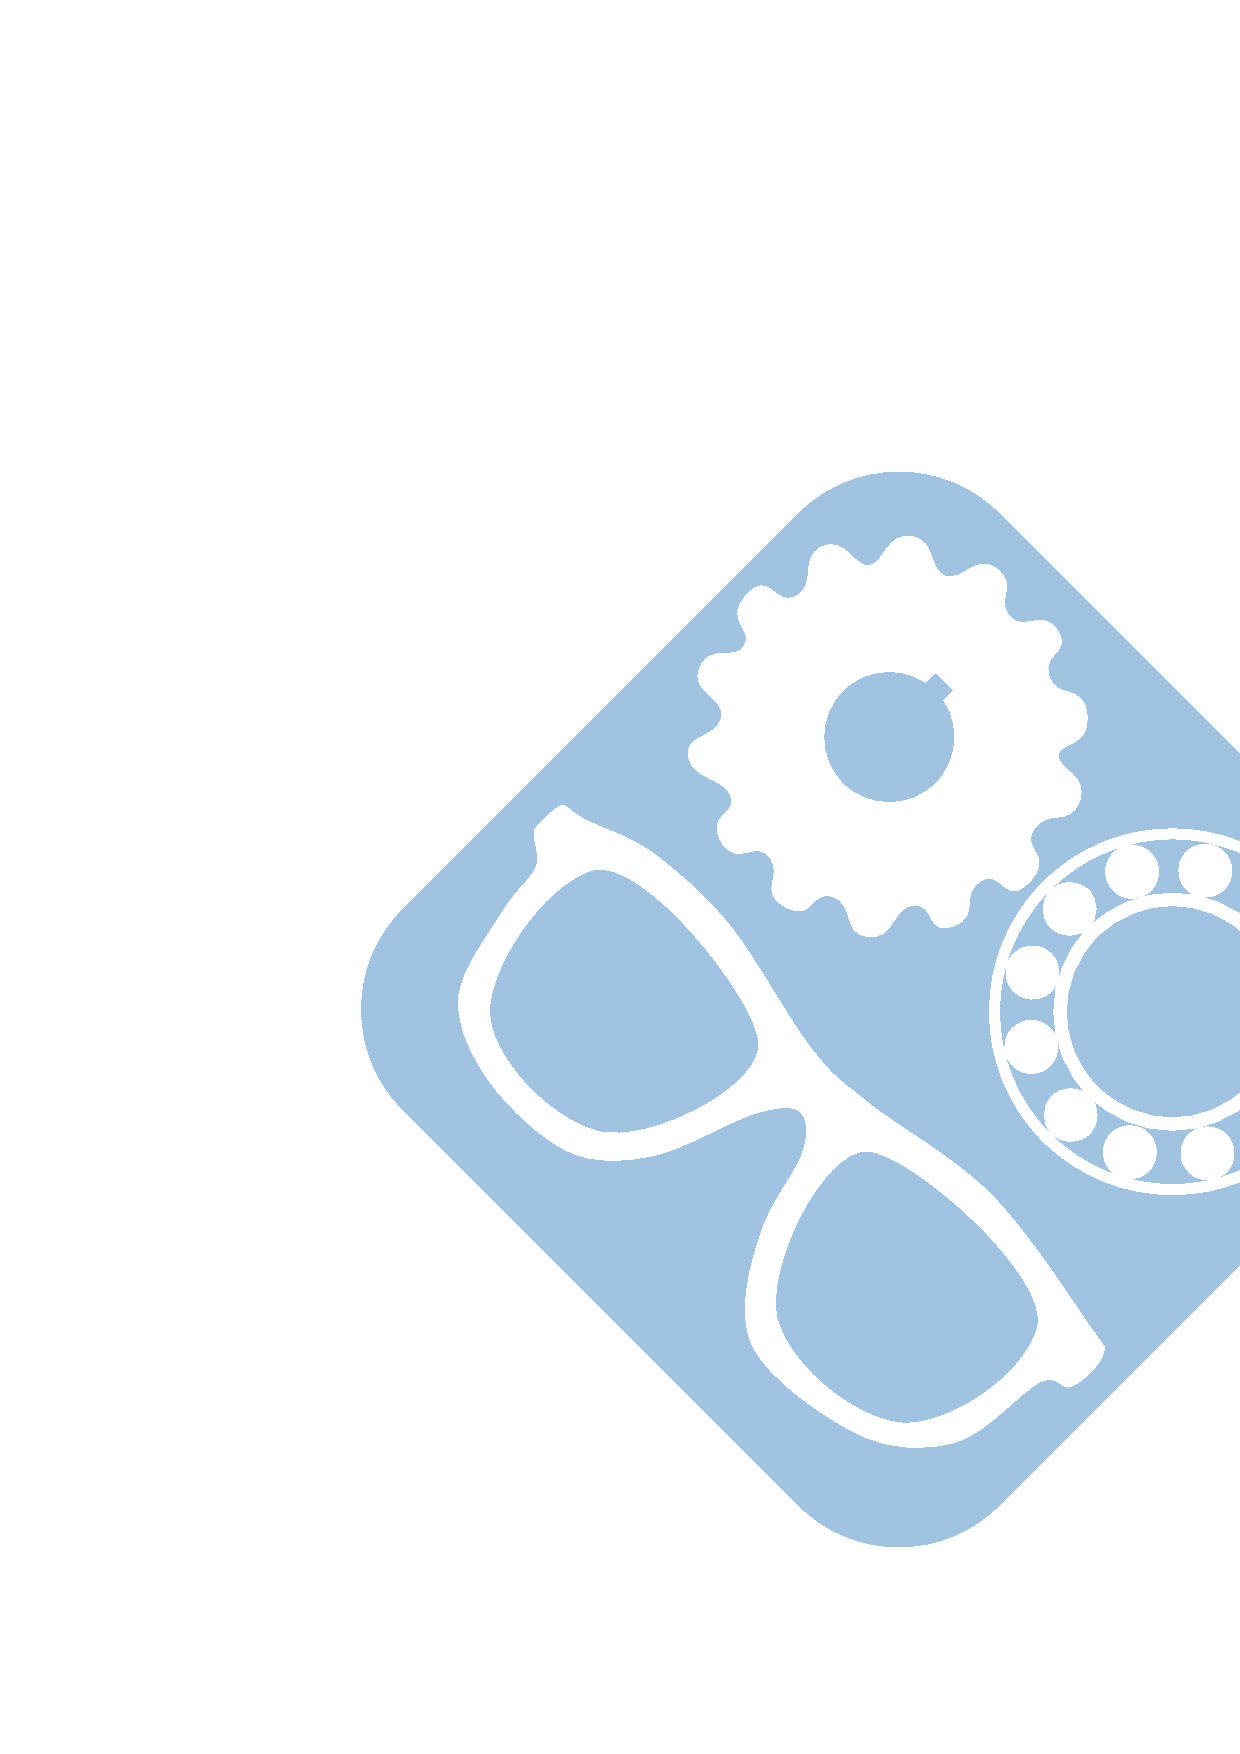
\includegraphics[width=\paperwidth,height=\paperheight,%
keepaspectratio]{../../../img/fond3}%
\end{center}
\vfill
}}}

\newcommand{\BackgroundPicdeux}{%
\put(25,-30){%
\parbox[b][\paperheight]{\paperwidth}{%
\vfill
\begin{center}
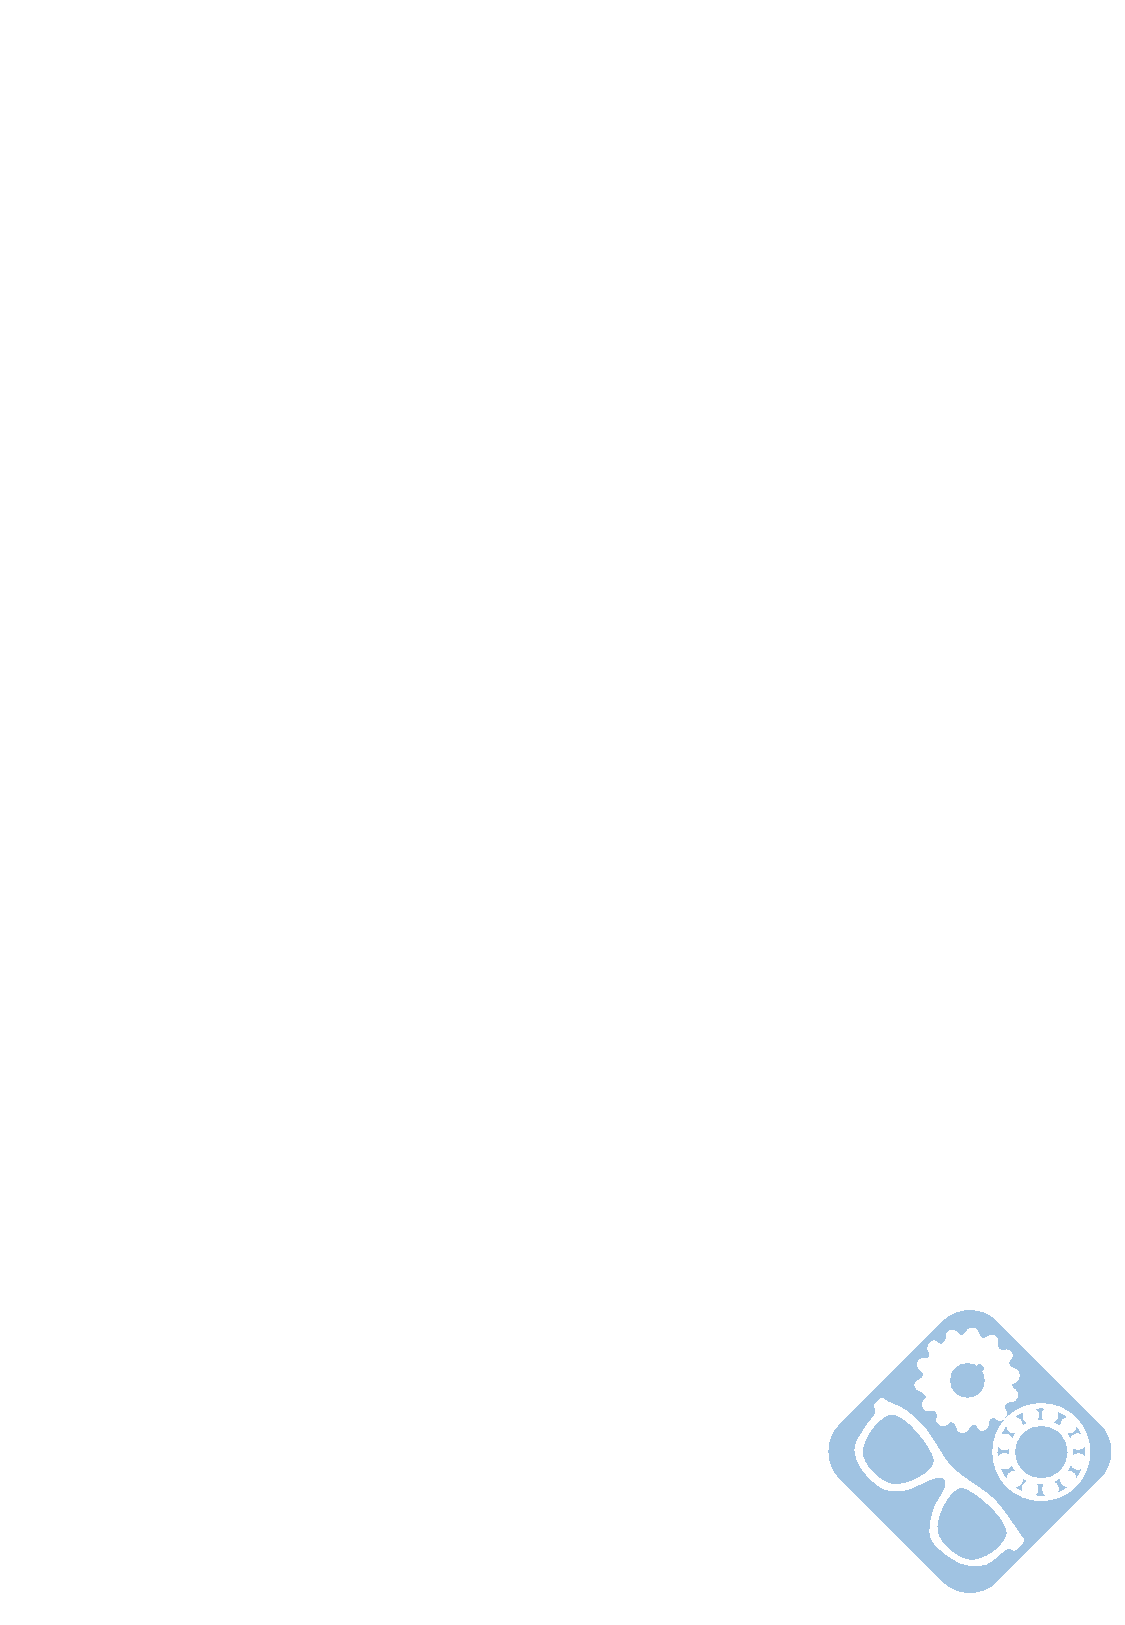
\includegraphics[width=\paperwidth,height=\paperheight,%
keepaspectratio]{../../../img/fond4}%
\end{center}
\vfill
}}}

\begin{document}

\pagestyle{empty}

\AddToShipoutPicture*{\BackgroundPic}


\includegraphics[width=2cm]{../../../img/logo}

\Huge{DS \numero - \sujet}

\vspace{1cm}

\ifdef{\prive}{\begin{center}\colorbox{danger}{\Huge{Avec Correction}}\end{center}}{}

\begin{center}
\centering\huge{PTSI}
\end{center}

\vspace{2cm}


\begin{center}
\centering\Large{\jour}
\end{center}

\vspace{2cm}

\normalsize

\tableofcontents

\newpage

\AddToShipoutPicture{\BackgroundPicdeux}

\pagestyle{fancy}

\begin{center}
\Huge \sujet
\end{center}


\normalsize


\section{Présentation}

\subsection{Contexte général}

La réalisation de composants ou empreintes d'outillage (injection plastique, tréfilage, découpage, estampage, ...) dans des matériaux de très grande dureté (aciers trempés, matériaux réfractaires, carbures et céramiques, ...) peut être limitée en utilisant des procédés conventionnels par enlèvement de matière tels que l'usinage à l'outil coupant (fraisage, tournage, perçage, ...) ou par abrasion (rectification, rodage,...). Une grande famille de procédés d'usinage permettant de répondre à certaines de ces exigences est associée aux techniques d'enlèvement de matière dites par électro-érosion (ou par
étincelage).

\subsection{Principe de l'électro-érosion}

\begin{figure}[!h]
 \centering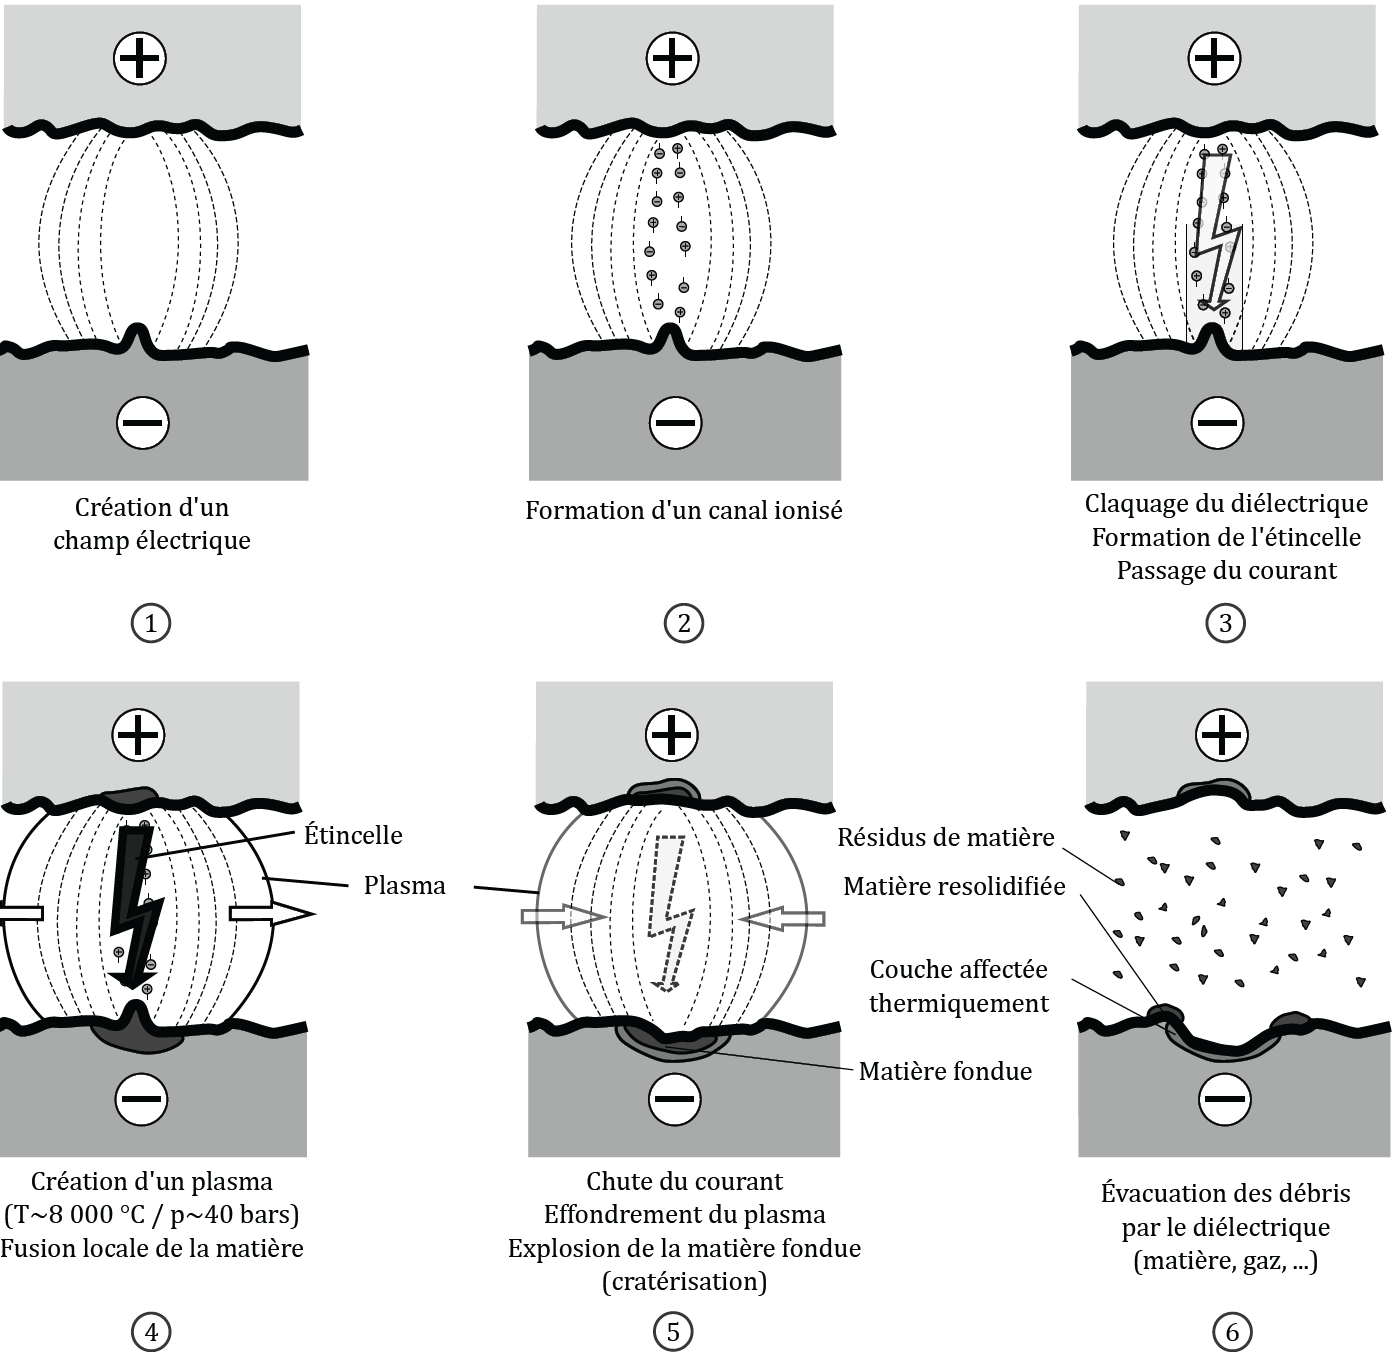
\includegraphics[width=0.8\linewidth]{img/img01}
 \caption{Les 6 étapes d'enlèvement de matière par électro-érosion}
 \label{img01}
\end{figure}

L'électro-érosion est un procédé d'usinage consistant à enlever de la matière par l'intermédiaire de décharges électriques entre deux électrodes immergées dans un fluide diélectrique (liquide ou gaz).

L'une des électrodes constitue l'outil et l'autre la pièce à usiner. La distance entre ces deux électrodes est appelée entrefer ou \textbf{gap}. L'effet des décharges électriques est le creusement de la pièce (et de l'usure de l'outil) par création d'un micro-plasma suivi de l'expulsion dans l'entrefer de débris provenant des deux électrodes. Le renouvellement du diélectrique dans l'entrefer et le rapprochement de l'outil et de la pièce permettent de redéfinir les conditions autorisant les nouvelles décharges. Par un
mouvement relatif de l'outil par rapport à la pièce, il est ainsi possible d'usiner progressivement la pièce tout en limitant l'usure de l'outil. On donne dans la figure \ref{img01} (page 2), les étapes successives d'enlèvement de matière par électro-érosion.

~\

On dénombre trois principaux procédés d'électro-érosion dont la représentation est donnée dans la figure \ref{img02} :
\begin{enumerate}
 \item l'électro-érosion par \textbf{enfonçage} consistant à déplacer verticalement l'électrode normalement à la surface à usiner (figure \ref{img02}a). On retire donc le négatif de la forme de l'électrode au gap près,
 \item l'électro-érosion à \textbf{fil fin} (figure \ref{img02}b), qui consiste à contourner, perpendiculairement à la surface (ou en inclinant légèrement le fil), le profil d'une pièce en déroulant un fil conducteur qui joue le rôle d'électrode,
 \item le \textbf{fraisage} par électro-érosion utilisé pour réaliser des formes par contournage ou des trous par enfonçage à l'aide d'électrodes cylindriques ou de formes. Cette technique est plutôt utilisée en micromécanique sous l'appellation de microfraisage ($\mu-EDM$ : Micro Electro-Discharge Machining) pour la réalisation de formes géométriques et l'utilisation d'électrodes de dimensions inférieures au millimètre (figure \ref{img02}c).
\end{enumerate}

~\

Ces trois techniques peuvent également être combinées pour la réalisation de composants.

\begin{figure}[!h]
 \centering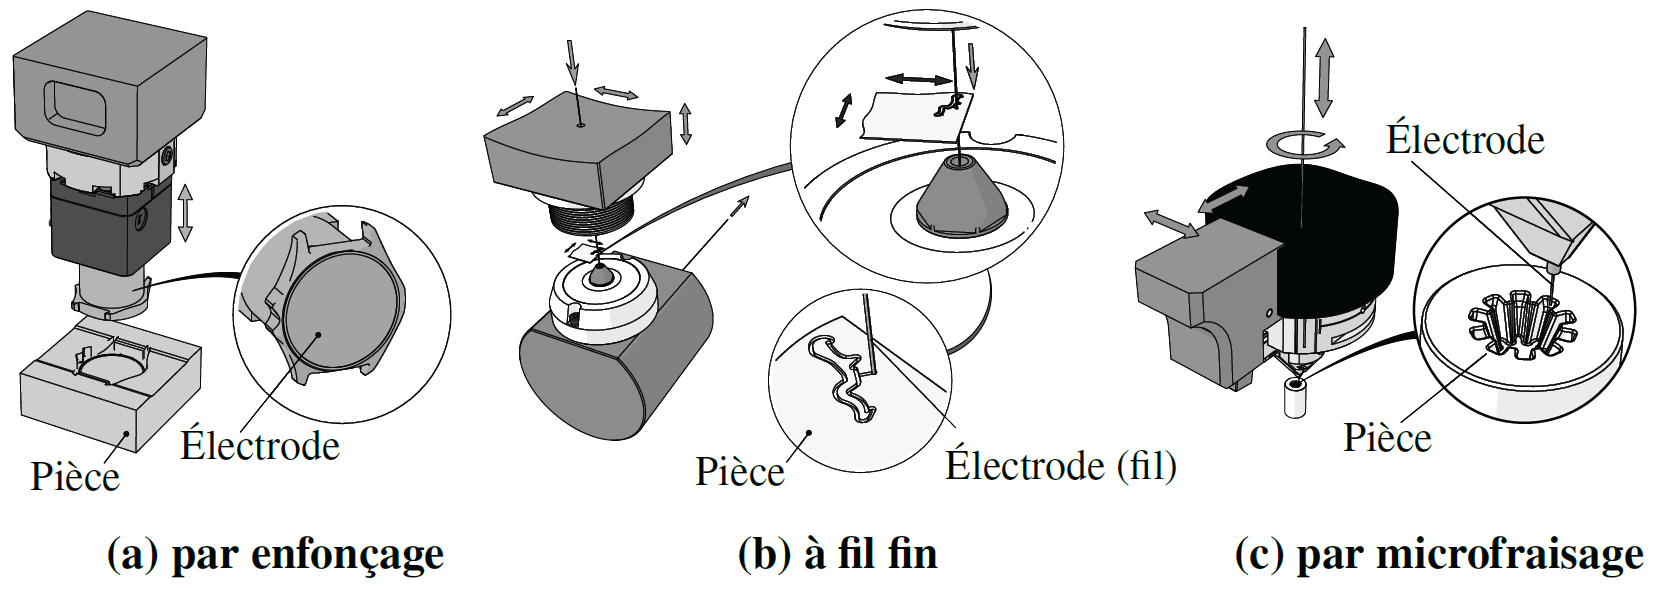
\includegraphics[width=0.9\linewidth]{img/img02}
 \caption{Les 3 grandes familles de procédés par électro-érosion}
 \label{img02}
\end{figure}

Dans le cadre de cette étude, on se concentre sur l'analyse d'une machine de microfraisage par érosion SARIX SX-200 telle que représentée dans la figure \ref{img03}a, en page 4, et plus particulièrement l'unité d'électro-érosion à fil appelée Arianne (figure \ref{img03}b).

\begin{figure}[!h]
 \centering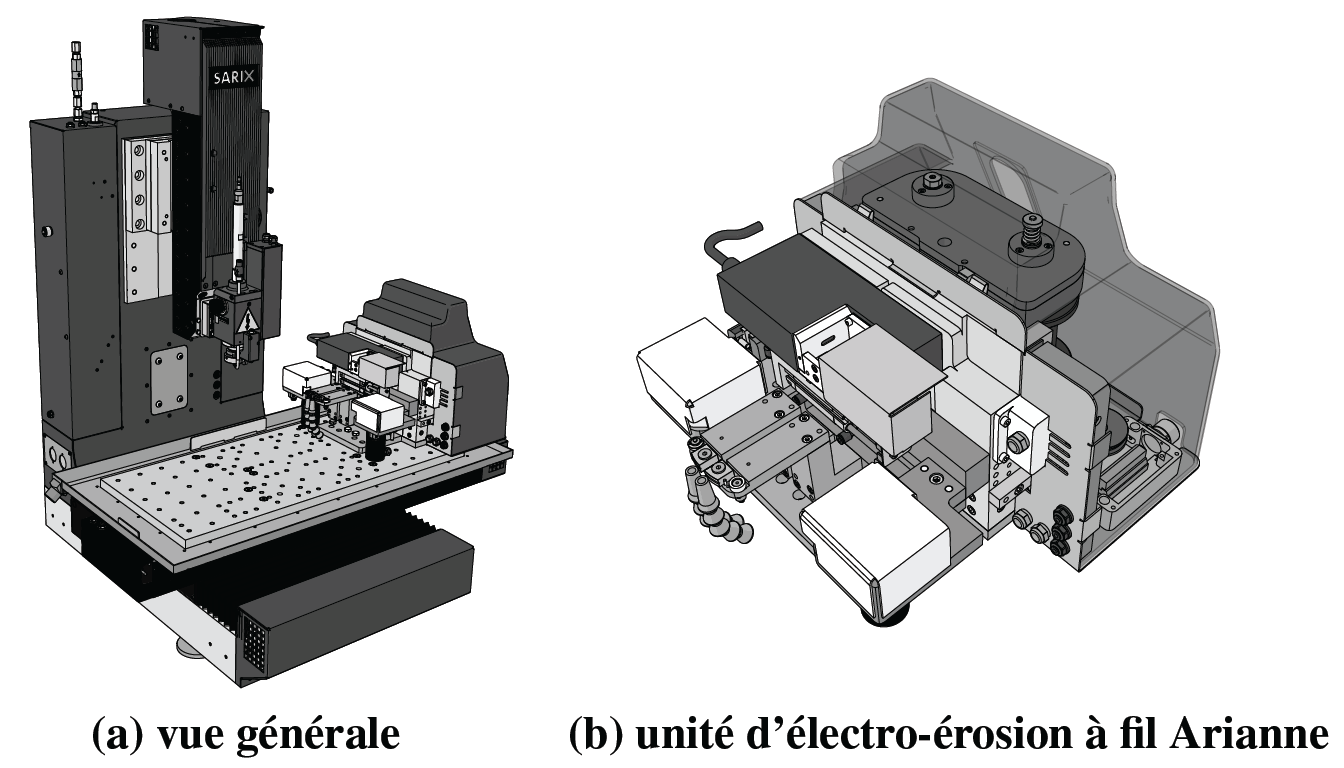
\includegraphics[width=0.9\linewidth]{img/img03}
 \caption{Machine de microfraisage par érosion SARIX SX-200}
 \label{img03}
\end{figure}

\newpage

\subsection{Unité d'électro-érosion à fil Arianne}

Le principe de l'unité à fil Arianne est d'utiliser le procédé d'électro-érosion à fil pour tailler à la forme et aux dimensions souhaitées les électrodes utilisées pour le microfraisage par érosion avec des tolérances serrées. Le principe de cette unité à fil est d'assurer le déroulement du fil en continu et à une vitesse constante $v_{fil}=5 mm\cdot s^{-1}$ dans la zone de taillage de l'électrode telle que représentée sur la figure \ref{img04}.

\begin{figure}[!h]
 \centering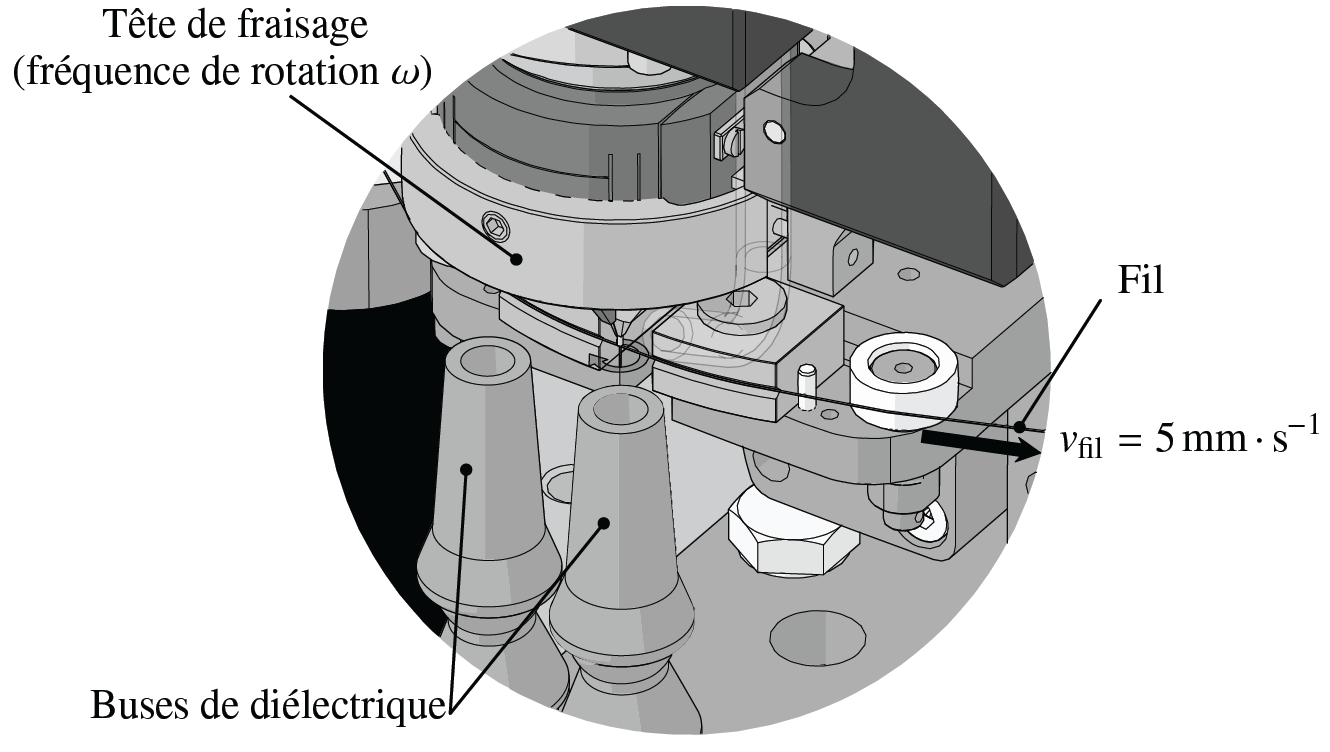
\includegraphics[width=0.7\linewidth]{img/img04}
 \caption{Unité d'électro-érosion à fil Arianne : zone de taillage}
 \label{img04}
\end{figure}

Le diagramme des exigences associé à l'unité à fil Arianne (Unité WEDM Arianne) est présenté dans le document 1 situé en page 1 de l'annexe.

Du point de vue des opérations de taillage, l'unité à fil est intégralement définie par les deux exigences 1.1 et 1.2. Une troisième exigence est quant à elle associée à la métrologie des électrodes réalisées tant sur les spécifications dimensionnelles que géométriques. Néanmoins, les exigences 1.1 et 1.2 doivent permettre de respecter les spécifications dimensionnelles et géométriques fixées, de l'ordre de quelques $\mu m$, sur la longueur, le diamètre et la forme de l'électrode.

L'objectif de ce sujet est de dimensionner ou de valider ces deux exigences. Afin de répondre à ces deux premières exigences, le système de la figure 5 est utilisé.

\begin{figure}[!h]
 \centering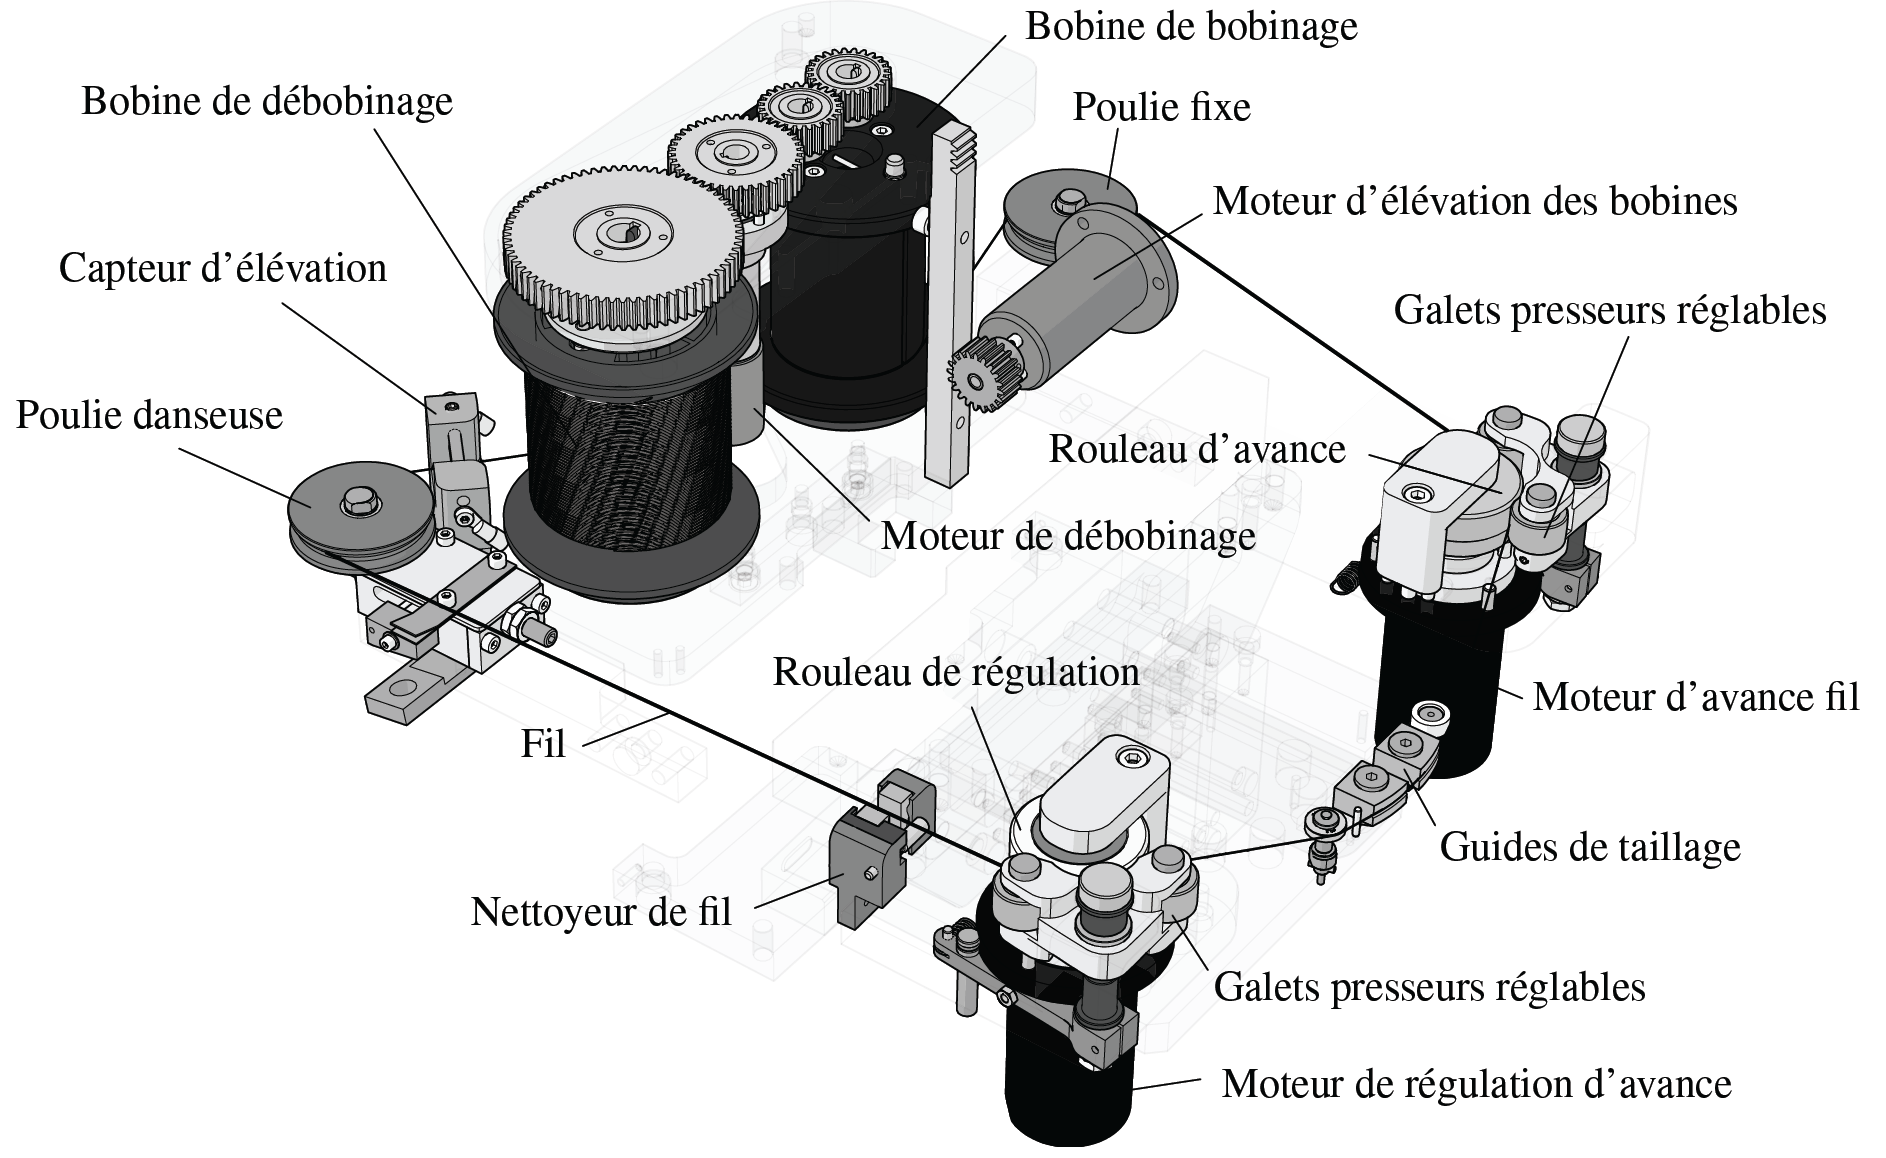
\includegraphics[width=0.9\linewidth]{img/img05}
 \caption{Unité d'électro-érosion à fil Arianne : système de défilement}
 \label{img05}
\end{figure}

\subsection{Principe de fonctionnement de l'unité Arianne}

Une \textbf{bobine de débobinage} de fil en alliage de cuivre de diamètre de $200\mu m$ est débobinée en amont de la zone de taillage à l'aide du \textbf{moteur de débobinage} par l'intermédiaire d'un train d'engrenages.

Ce moteur assure également la récupération du fil utilisé en aval du taillage sur la \textbf{bobine de bobinage} par l'intermédiaire d'un second train d'engrenages. Le fil est alors déroulé entre deux armatures conductrices d'un \textbf{capteur} dit \textbf{d'élévation} permettant de contrôler l'horizontalité du fil déroulé.

Lorsque le fil est en contact avec l'une des deux armatures, un système de régulation active un \textbf{moteur d'élévation des bobines} en liaison avec un système pignon-crémaillère déplaçant verticalement le bloc constitué des bobines, du moteur de débobinage et des trains d'engrenages. Le fil se déroule ainsi toujours dans le même plan.

Le fil est ensuite guidé par une \textbf{poulie danseuse} se déplaçant en fonction de la tension du fil en sortie de bobine. Ce déplacement est assuré par un \textbf{capteur inductif} (non représenté sur la figure) utilisé pour contrôler la vitesse de rotation du moteur de débobinage et donc la vitesse de déroulement du fil. La régulation en vitesse et en tension (mécanique) du fil s'opère à l'aide de deux moteurs pilotés en courant et montés sur les axes de deux \textbf{rouleaux} (cabestans). Le \textbf{moteur d'avance fil} donne le mouvement d'avance au fil par l'intermédiaire du \textbf{rouleau d'avance}. Le fil est maintenu en contact sur ce rouleau à l'aide d'un système à \textbf{galets presseurs réglables}. La vitesse du fil est quant à elle régulée par l'intermédiaire d'un système équivalent à l'aide d'un \textbf{moteur de régulation} en liaison directe avec un \textbf{rouleau de régulation}. La régulation en courant de ces deux moteurs permet ainsi de contrôler la vitesse moyenne du fil dans la zone de taillage et également de contrôler la tension dans
le fil.

Le taillage des électrodes est alors assuré entre ces deux systèmes par des \textbf{guides de taillage} espacés d'une distance dtail. Cette zone est décalée par rapport aux systèmes d'avance fil et de régulation de l'avance afin d'assurer une pré-tension dans le fil dans la zone de taillage.

Une fois le fil déroulé et utilisé en sortie de zone de taillage et du système d'avance fil, le fil est mené par la \textbf{poulie fixe} vers la \textbf{bobine de bobinage}.

\section{Détermination des spécifications du système}

Objectifs:
\begin{itemize}
 \item Déterminer le matériau constitutif du fil,
 \item Choisir un moteur à courant continu et le modulateur associé,
 \item Valider la régulation en vitesse du banc d'essai.
\end{itemize}

\subsection{Détermination du matériau constitutif du fil}

L'utilisation de fils en alliage de cuivre de type laiton (CuZn), bronze (CuSn), Cupro-nickel (CuNi)ou Cuivre-Fer (CuFe) est motivée par les propriétés électriques et mécaniques de ce type d'alliage pour l'application visée. Dans le cas de l'unité de taillage Arianne, il est nécessaire que le fil utilisé dispose d'une grande conductibilité électrique afin d'assurer le taillage de l'électrode. Celle-ci doit être au minimum de 20\% de l'IACS (International Annealed Copper Standard). La valeur de 100%
de l'IACS correspond à la conductibilité maximale du cuivre pur. Le système de régulation en vitesse contrôle également la tension mécanique du fil lors du procédé de taillage, l'alliage doit donc disposer d'une importante résistance à la traction (supérieure à $500N\cdot mm^{-2}$). De plus, pour des considérations de recyclage et de réponse à la norme environnementale REACH, les alliages disposant de plomb (Pb) ou de nickel (Ni) doivent être proscrits. Enfin, d'un point de vue économique, on tendra à choisir le matériau le moins cher.

\question{À l'aide du document 2 de l'annexe, déterminer en justifiant l'alliage de cuivre répondant aux différents critères énoncés.}

\subsection{Validation du moteur}

La bobine de débobinage admet un diamètre Ddeb variant de 7,2 cm (pleine) à 5 cm (vide).

On donne dans la figure 6 de la page 7, le schéma cinématique du système permettant l'actionnement du débobinage/récupération du fil. Le moteur 1 développe un couple Cm à la vitesse de rotation $\omega_m$. Il est relié à un réducteur épicycloïdal 2 dont le rapport est $k_r=\frac{1}{415}$. En sortie de réducteur, un pignon 3 disposant de $Z_{mr}=40$ dents engrène deux pignons. Le premier pignon 4 est directement relié à la bobine de débobinage et dispose de $Z_{deb}=69$ dents. Le second est un pignon inverseur 5, disposant de $Z_{pi}=25$ dents, engrène quant à lui le pignon 6 relié à la bobine de bobinage disposant également de $Z_{bob}=25$ dents. On considérera que les engrènements se font dans l'hypothèse de roulement sans glissement.

\newpage

\begin{figure}[!h]
 \centering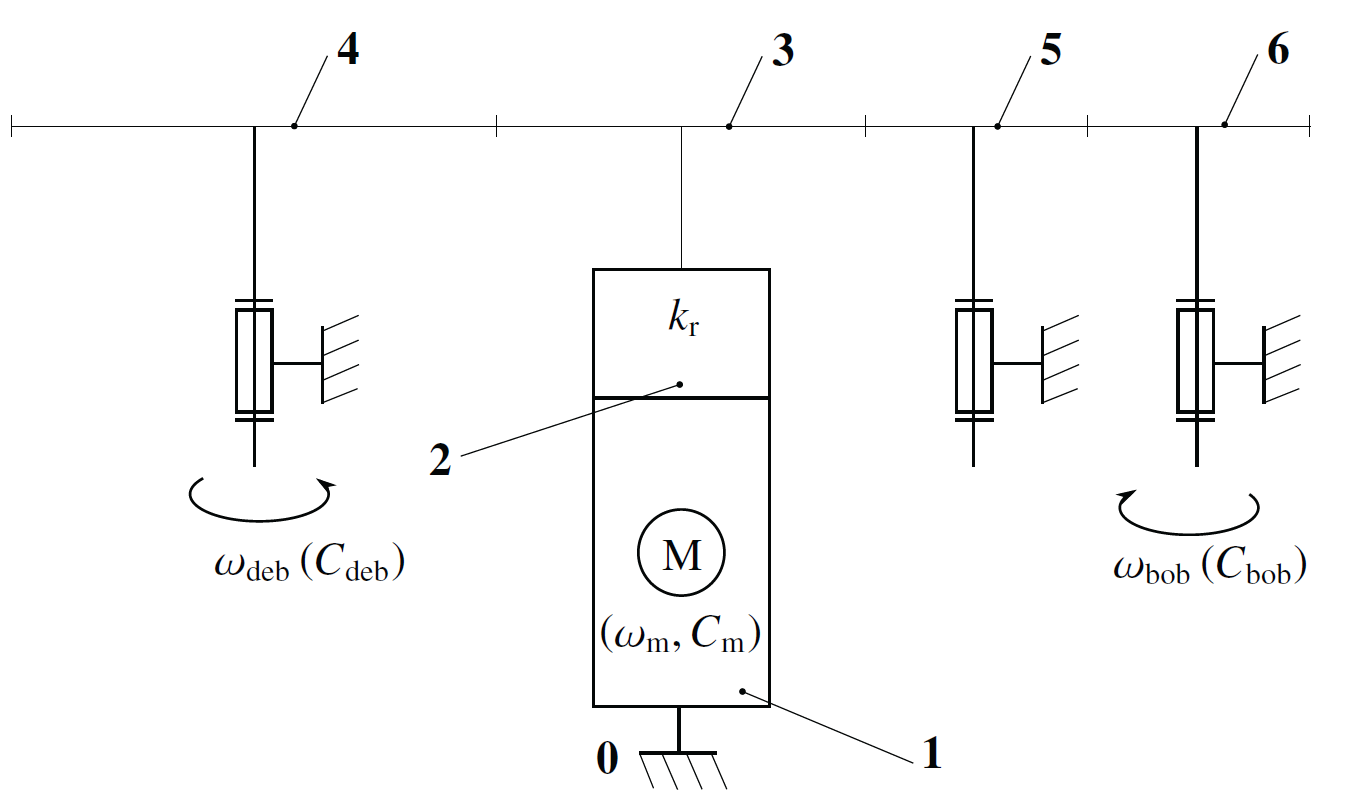
\includegraphics[width=0.7\linewidth]{img/img06}
 \caption{Schéma cinématique du système de débobinage/récupération}
 \label{img06}
\end{figure}

Une première étude sur la chaine de transmission a permis de montrer que:
\begin{center}
$C_m=\frac{k_r}{\eta_r}\cdot\left(C_{deb}.\frac{Z_{mr}}{Z_{deb}}+C_{bob}.\frac{Z_{mr}}{Z_{bob}}\right)$,
\end{center}


Avec:\\
\begin{center}
$\left\{\begin{array}{c}
2,1 N\cdot m < C_{deb} < 2,7 N\cdot m \\
0,8 N\cdot m < C_{bob} < 1,2 N\cdot m
\end{array}\right.$
\end{center}

On supposera que les engrènements se font sans pertes, seul le réducteur 2 a un rendement \\$\eta r=0,48$.

Le couple moteur utile est donc compris entre deux valeurs limites $C_{m\ min}$ et $C_{m\ max}$ tel que :
\begin{center}
$C_{m\ min} < C_m < C_{m\ max}$
\end{center}

\question{Déterminer les valeurs limites $C_{m\ min}$ et $C_{m\ max}$.}

~\

Pour la suite, on supposera que $12 mN\cdot m < Cm < 18 mN\cdot m$ et $100 rad\cdot s^{-1} < \omega_m < 143 rad.s^{-1}$.

~\

On supposera également que l'alimentation électrique présente peut fournir une tension comprise entre 0 et 24 V.

~\

Les caractéristiques du moteur 2232 024 SR de la société Faulhaber utilisé sont données dans le tableau 1.

\begin{table}
\begin{center}
\begin{tabular}{|c|c|}
\hline
Caractéristique & Valeur \\
\hline
Tension nominale & $U_n = 24V$ \\
\hline
Puissance utile & $Pu = 8,68W$ \\
\hline
Rendement maximal & $\eta_{max} = 86\%$ \\
\hline
Inductance d'induit & $L = 710 \mu H$ \\
\hline
Résistance d'induit & $R = 16\Omega$ \\
\hline
Constante de force électromotrice & $k_e = 32 mV\cdot rad^{-1}\cdot s$ \\
\hline
Constante de couple & $k_t = 32 mN\cdot m\cdot A^{-1}$ \\
\hline
%Couple de frottement sec & $C_f = 1mN\cdot m$ \\
%\hline
Moment d'inertie du rotor & $J = 6,4 g\cdot cm^2$ \\
\hline
Température maximale admissible & $Tmax = 125 \textdegree C$ \\
\hline
Résistance thermique entre le bobinage de l'induit et le boitier & $Rth1 = 3 \degree C\cdot W^{-1}$ \\
\hline
Résistance thermique entre le boitier et l'air ambiant & $Rth2 = 11 \degree C\cdot W^{-1}$ \\
\hline
Fréquence de rotation nominale & $Nn = 5 480 tr\cdot min^{-1}$ \\
\hline
Couple nominal & $Cn = 10 mN\cdot m$ \\
\hline
Courant nominal & $In = 0,33A$ \\
\hline
\end{tabular}
 \caption{Caractéristiques du moteur 2232 024 SR de la société Faulhaber}
 \label{tab01}
 \end{center}
\end{table}

\newpage

\question{Vérifier que le moteur 2232 024 SR de la société Faulhaber choisi peut fournir la puissance ($P_{meca}=C_m.\omega_m$)
requise.}

~\

En fonctionnement normal, le couple moteur est supérieur au couple nominal $C_n = 10mN\cdot m$ de ce moteur, il convient alors de vérifier que l'échauffement du bobinage ne sera pas excessif. Pour cela, il faut déterminer la température du bobinage dans le cadre du fonctionnement étudié.

Le modèle électrique retenu pour l'induit du moteur à courant continu est donné figure \ref{img08}.


\begin{figure}[!h]
 \centering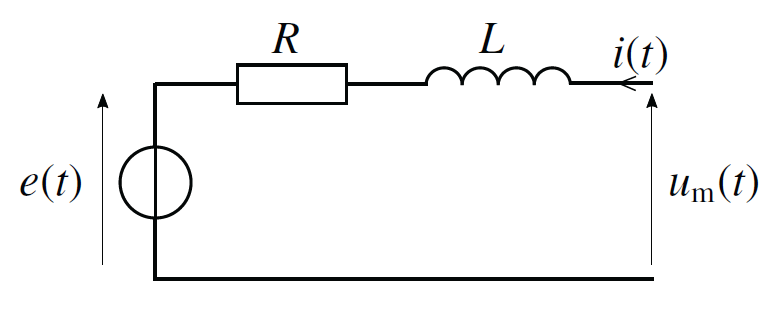
\includegraphics[width=0.6\linewidth]{img/img08}
 \caption{Modèle électrique du moteur à courant continu}
 \label{img08}
\end{figure}

\question{Donner l'équation électrique vérifiée par la tension instantanée de l'induit du moteur $u_m(t)$.
Que devient cette équation en régime permanent stabilisé, c'est-à-dire lorsque $u_m(t)=U_m$,
$e(t)=E_m$, $i(t)=I_m$ et $\omega_m(t)=\Omega_m$ sont constants ?}

\question{Pour le couple moteur maximal $C_{m\ max}$ de $18mN\cdot m$, et en vous aidant des autres équations du moteur électrique, déterminer le courant absorbé maximal par ce moteur $I_{max}$ et les pertes par effet Joule maximales $P_{j\ max}$.}

~\

On prendra pour la suite $P_{j\ max}=5,5W$.

\newpage

Une étude de comportement thermique a permis de déterminer la relation suivante:
\begin{center}
$T_{bobinage}=T_{amb}+P_{j\ max}\cdot (R_{th1}+R_{th2})$.
\end{center}

avec:
\begin{itemize}
 \item $P_j$, pertes par effet Joule de l'induit du moteur (on néglige les autres pertes du moteur),
 \item $T_{bobinage}$, température du bobinage de l'induit,
 \item $T_{boitier}$, température du boitier,
 \item $T_{amb}$, température de l'air ambiant, $T_{amb}=40\degree C$,
 \item $R_{th1}$, résistance thermique entre le bobinage et le boitier,
 \item $R_{th2}$, résistance thermique entre le boitier et l'air ambiant.
\end{itemize}

\question{Justifier que l'on puisse valider le choix du moteur 2232 024 SR de la société Faulhaber.}

\subsection{Réponse temporelle du moteur}

\question{Donner les 4 équations qui décrivent le comportement du moteur électrique à courant continu:
\begin{itemize}
 \item équation électrique,
 \item équation mécanique (P.F.D) sans couple résistant et les frottements sont négligés,
 \item couplage force électromotrice/vitesse de rotation,
 \item couplage couple/courant,
\end{itemize}}

\question{Écrire ces équations dans le domaine de Laplace.}

\question{En déduire la forme canonique de la fonction de transfert du moteur $H(p)=\frac{\Omega_m(p)}{U_m(p)}$. Donner son ordre, sa classe, et la forme littérale de ses constantes caractéristiques.}

\question{Faire les applications numériques.}

~\

Pour la suite, on prendra $K=30V^{-1}\cdot rad\cdot s^{-1}$, $\xi=8$ et $\omega_0=1400rad.s^{-1}$.

\question{Justifier qu'il est possible de la mettre sous la forme suivante:

\begin{center}
$H(p)=\frac{K_1}{(1+T_1\cdot p)\cdot (1+T_2\cdot p)}$.
\end{center}

En déduire $K_1$, $T_1$ et $T_2$. On prendra $\sqrt{63}=7,94$.}

\question{Justifier qu'il est alors possible de la mettre sous la forme suivante:

\begin{center}
$H(p)=\frac{K_2}{(1+\tau\cdot p)}$.
\end{center}

En déduire $K_2$ et $\tau$.}

~\

Le document 4 des annexes donne la réponse temporelle de la vitesse de rotation $\Omega(t)$.

\question{Ce tracé correspond-t-il à vos attentes ? Décrire alors l'entrée (type d'entrée et valeur numérique) qui a du être utilisée pour arriver à ce tracé.}

~\

Le moteur étudié précédemment est alors utilisé dans un asservissement dont la Fonction de Transfert en Boucle Fermée (FTBF) est donnée en annexe document 5.

\question{Préciser l'ordre et la classe de cette FTBF. En déduire des valeurs approchées de ses constantes caractéristiques.}

Pour effectuer ces applications numériques, on pourra utiliser les données suivantes:
\begin{itemize}
 \item $\left(ln\left(\frac{1}{17}\right)\right)^2\approx 8$,
 \item $\pi^2\approx 10$,
 \item $ln(20)\approx 3$,
\end{itemize}

\section{Etude basculeur}

Le dessin de définition d'un basculeur est donné dans le document réponse.

\question{Colorier les classes d'équivalence de ce système.}

\newpage
\cleardoublepage

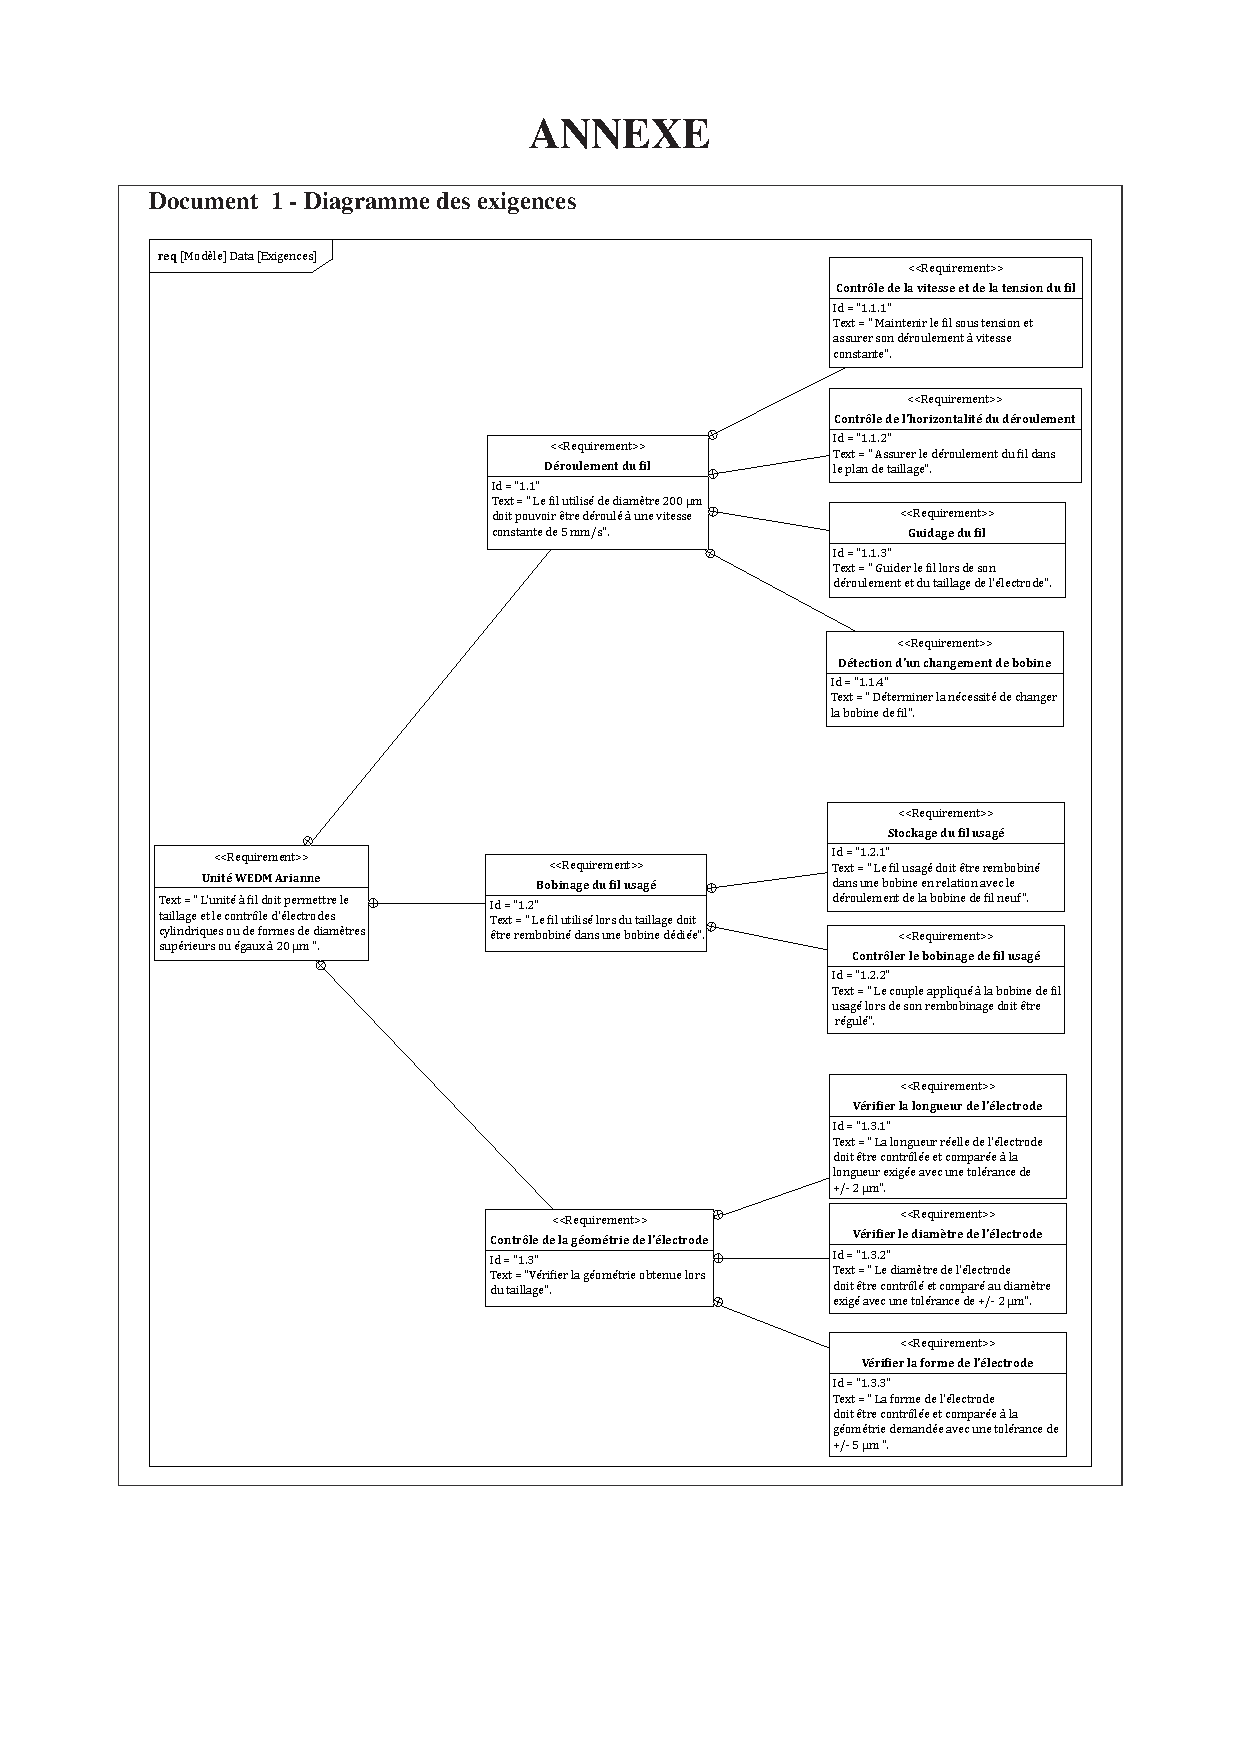
\includepdf[offset=5mm -10mm 0mm 0mm,pages=1]{img/annexes.pdf}
\includepdf[offset=-5mm -10mm 0mm 0mm,pages=2]{img/annexes.pdf}
\includepdf[offset=10mm 0mm 0mm 0mm,pages=3]{img/annexes.pdf}
\includepdf[offset=-10mm -10mm 0mm 0mm,pages=4]{img/annexes.pdf}
\includepdf[offset=10mm -10mm 0mm 0mm,pages=5]{img/annexes.pdf}
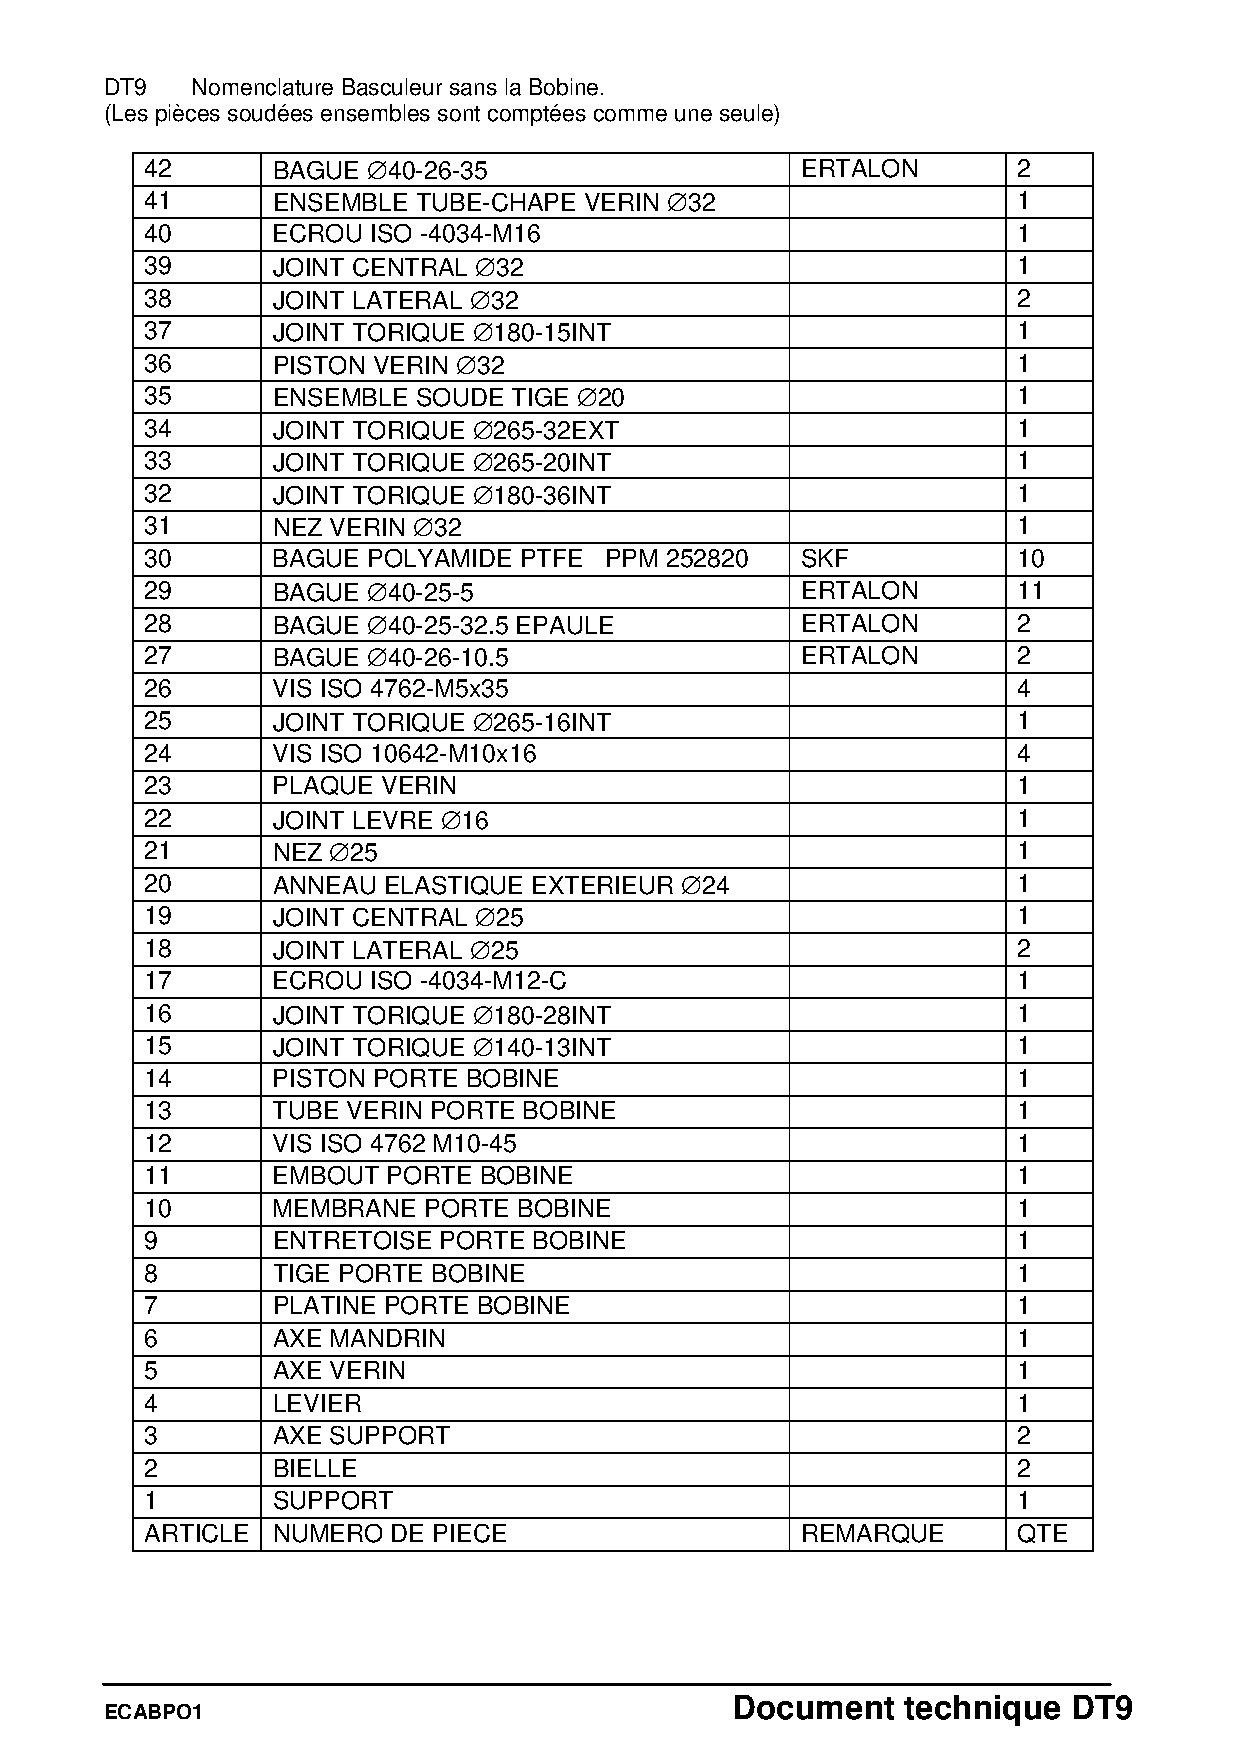
\includepdf[offset=5mm -10mm 0mm 0mm,pages=1]{img/annexes_2.pdf}

\newpage
\cleardoublepage

\pagestyle{documentreponse}


\section{Documents réponse}

\reponse{1}{\ifdef{\public}{\vspace{4cm}}{A partir du document 2, on isole CuZn30 et CuZn36, le moins cher étant CuZn36, c'est celui que l'on sélectionne.}}

\reponse{1}{\ifdef{\public}{\vspace{9cm}}{$C_{m\ min}=\frac{1}{415\cdot 0,48}\cdot \left(2,1\cdot \frac{40}{69}+0,8\cdot \frac{40}{25}\right)=12,5mN\cdot m$ \\
$C_{m\ max}=\frac{1}{415\cdot 0,48}\cdot \left(2,7\cdot \frac{40}{69}+1,2\cdot \frac{40}{25}\right)=17,5mN\cdot m$
}}

\reponse{1}{\ifdef{\public}{\vspace{6cm}}{$P_{meca}=C_m.\omega_m=0,018\cdot 143=2,5W<8,68W$, donc le moteur convient.}}

\ifdef{\public}{\newpage}{}

\reponse{1}{\ifdef{\public}{\vspace{6cm}}{$u_m(t)=R.i(t)+L\frac{di(t)}{dt}+e(t)$, ce qui devient $U_m=R.I_m+E_m$ lorsque les coefficients sont constants.}}

\reponse{1}{\ifdef{\public}{\vspace{6cm}}{$c_m(t)=k_t.i(t)$, ce qui devient $C_{m\ max}=k_t.I_{max}$, donc $I_{max}=\frac{C_{m\ max}}{k_t}=\frac{18\cdot 10^{-3}}{32\cdot 10^{-3}}\approx 0,6$, donc $P_{j\ max}=R.I_{max}^2=16\cdot 0,6^2=16\cdot 0,36\approx 5,5W$.}}

\reponse{1}{\ifdef{\public}{\vspace{8cm}}{$T_{bobinage}=40+5,5\cdot (3+11)=40+77=117\degree C<125\degree C$, donc le moteur convient.}}

\ifdef{\public}{\newpage}{}

\reponse{1}{\ifdef{\public}{\begin{itemize} \item ~\ \\ \item ~\ \\ \item ~\ \\ \item ~\ \end{itemize}}{\begin{itemize}\item $u_m(t)=R\cdot i(t)+L\frac{di(t)}{dt}+e(t)$,\\ \item $c_m(t)=k_t\cdot i(t)$,\\ \item $e(t)=k_e\cdot \omega_m(t)$, \\ \item $J\cdot \frac{d\omega_m(t)}{dt}=C_m(t)$.\end{itemize}}}

\reponse{1}{\ifdef{\public}{\begin{itemize} \item ~\ \\ \item ~\ \\ \item ~\ \\ \item ~\ \end{itemize}}{\begin{itemize}\item $U_m(p)=R\cdot I(p)+L\cdot p\cdot I(p)+E(p)$,\\ \item $C_m(p)=k_t\cdot I(p)$,\\ \item $E(t)=k_e\cdot \Omega_m(p)$,\\ \item $J\cdot p\cdot \Omega_m(p)=C_m(p)$.\end{itemize}}}

\reponse{1}{\ifdef{\public}{\vspace{2cm} H(p)= \\ classe: \\ ordre: \\ constantes caractéristiques: \vspace{4cm}}{$U_m(p)=((R+L\cdot p)\cdot \frac{J\cdot p}{k_t}+k_e).\Omega_m(p)$, donc $H(p)=\frac{\Omega_m(p)}{U_m(p)}=\frac{1}{(R+L\cdot p)\cdot \frac{J\cdot p}{k_t}+k_e}=\frac{\frac{1}{k_e}}{1+\frac{R\cdot J}{k_e\cdot k_t}\cdot p+\frac{L\cdot J}{k_e\cdot k_t}\cdot p^2}$. \\ C'est un fonction de classe 0 et d'ordre 2. Ses constantes caractéristiques sont $K=\frac{1}{k_e}$, $\omega_0=\sqrt{\frac{k_e\cdot k_t}{L\cdot J}}$ et $\xi=\frac{R}{2}\cdot \sqrt{\frac{J}{k_e\cdot k_t\cdot L}}$.}}

\reponse{1}{\ifdef{\public}{\vspace{3cm}}{$K=\frac{1}{k_e}=\frac{1}{32\cdot 10^{-3}}=\frac{1000}{32}\approx 30$.\\$\omega_0=\sqrt{\frac{k_e\cdot k_t}{L\cdot J}}=\sqrt{\frac{32^2\cdot 10^{-6}}{710\cdot 10^{-6}\cdot 64\cdot 10^{-8}}}=\sqrt{\frac{32^2\cdot 10^8}{710\cdot 64}}=\sqrt{\frac{16}{710}}\cdot 10^	4\approx\sqrt{\frac{16}{800}}\cdot 10^4\approx\sqrt{2}\cdot 10^3\approx1400rad.s^{-1}$.\\$\xi=\frac{R}{2}\cdot \sqrt{\frac{J}{k_e\cdot k_t\cdot L}}=\frac{16}{2}\cdot \sqrt{\frac{64\cdot 10^{-8}}{32^2\cdot 10^{-6}\cdot 710\cdot 10^{-6}}}=8\cdot \sqrt{\frac{10^4}{16\cdot 710}}\approx 8\cdot \sqrt{\frac{10^4}{16\cdot 700}}\approx 8\cdot \sqrt{\frac{10^4}{11200}}\approx 8\cdot \sqrt{\frac{10}{11,2}}\approx 8$.}}

\ifdef{\public}{\newpage}{}

\reponse{1}{\ifdef{\public}{Justifications:\\ \vspace{2cm}\\ $K_1=$ \\ $T_1=$ \\ $T_2=$\\ }{$\xi\approx 8>1$, donc il existe deux racines réelles négatives, donc il est possible d'écrire la fonction de transfert sous la forme proposée.

$K_1=K$

Racines du polynôme: $1+2\cdot \frac{\xi}{\omega_0}\cdot p+\frac{p^2}{\omega_0^2}=0$

$\Delta=\frac{4\cdot \xi^2}{\omega_0^2}-\frac{4}{\omega_0^2}=\frac{4\cdot(\xi^2-1)}{\omega_0^2}$

$p_1=\frac{-\frac{2\cdot \xi}{\omega_0}-\sqrt{\frac{4\cdot(\xi^2-1)}{\omega_0^2}}}{\frac{2}{\omega_0^2}}=\omega_0\cdot(-\xi-\sqrt{\xi^2-1})\approx1400\cdot(-8-\sqrt{63})\approx1400\cdot(-8-7,94)\approx -1400\cdot 15,94\approx -22400$, donc $T_1=-\frac{1}{p_1}\approx4,4\cdot10^{-5}s$\\

$p_2=\frac{-\frac{2\cdot \xi}{\omega_0}+\sqrt{\frac{4\cdot(\xi^2-1)}{\omega_0^2}}}{\frac{2}{\omega_0^2}}\approx1400\cdot(-8+\sqrt{63})\approx1400\cdot (-8+7,94)\approx-1400\cdot 0,06\approx -84$, donc $T_2=0,01s$.}}

\reponse{1}{\ifdef{\public}{Justifications:\\ \vspace{2cm}\\ $K_2=$ \\ $\tau=$\\ }{$T_1<<T_2$, donc on peut écrire la fonction $H(p)$ sous la forme proposée avec $K_2=K$ et $\tau=T_2=0,01s$.}}

\reponse{1}{\ifdef{\public}{\vspace{4cm}}{Ce tracé est celui d'un premier ordre avec une entrée en échelon (tangente à l'origine non nulle, avec une pente qui coupe l'asymptote à un temps correspondant au tiers du temps de réponse à 5\%). La valeur limite est $\omega_m(+\infty)=120rad.s^{-1}$, donc $U_0=120\cdot 32\cdot 10^{-3}\approx 3,8V$. Le temps de réponse à 5\% est environ de 0,03s ce qui correspond à $3\cdot \tau$ avec $\tau=0,01s$, comme trouvé à la question précédente.}}


\reponse{1}{\ifdef{\public}{\vspace{2cm}}{On voit un dépassement sur le tracé donc il s'agit d'un second ordre avec $\xi<1$.

Le dépassement vaut: $D\%=100\cdot \frac{0,9-0,85}{0,9}=\frac{100}{17}=100\cdot e^{-\frac{\xi\cdot \pi}{\sqrt{1-\xi^2}}}$, donc 

$ln\left(\frac{1}{17}\right)=-\frac{\xi\cdot \pi}{\sqrt{1-\xi^2}}$ 

$\left(ln\left(\frac{1}{17}\right)\right)^2=\frac{\xi^2\cdot \pi^2}{1-\xi^2}$ 

$\left(ln\left(\frac{1}{17}\right)\right)^2\cdot \left(1-\xi^2\right)=\xi^2\cdot \pi^2$ 

$8=\xi^2\cdot (10+8)$

$\xi=\sqrt{\frac{8}{18}}\approx\sqrt{\frac{9}{18}}\approx\frac{1}{1,4}\approx0,6$
 
$t_{R5\%}=\frac{1}{\xi\cdot \omega_0}\cdot ln(20)=0,012s$ d'après le graphique.

Donc $\omega_0=\frac{1}{\xi\cdot t_{R5\%}}\cdot ln(20)\approx\frac{1}{0,6\cdot 0,012}\cdot ln(20)\approx\frac{3}{6\cdot 12\cdot 10^{-4}}\approx\frac{10^4}{24}\approx500rad.s^-1$.}}

\ifdef{\public}{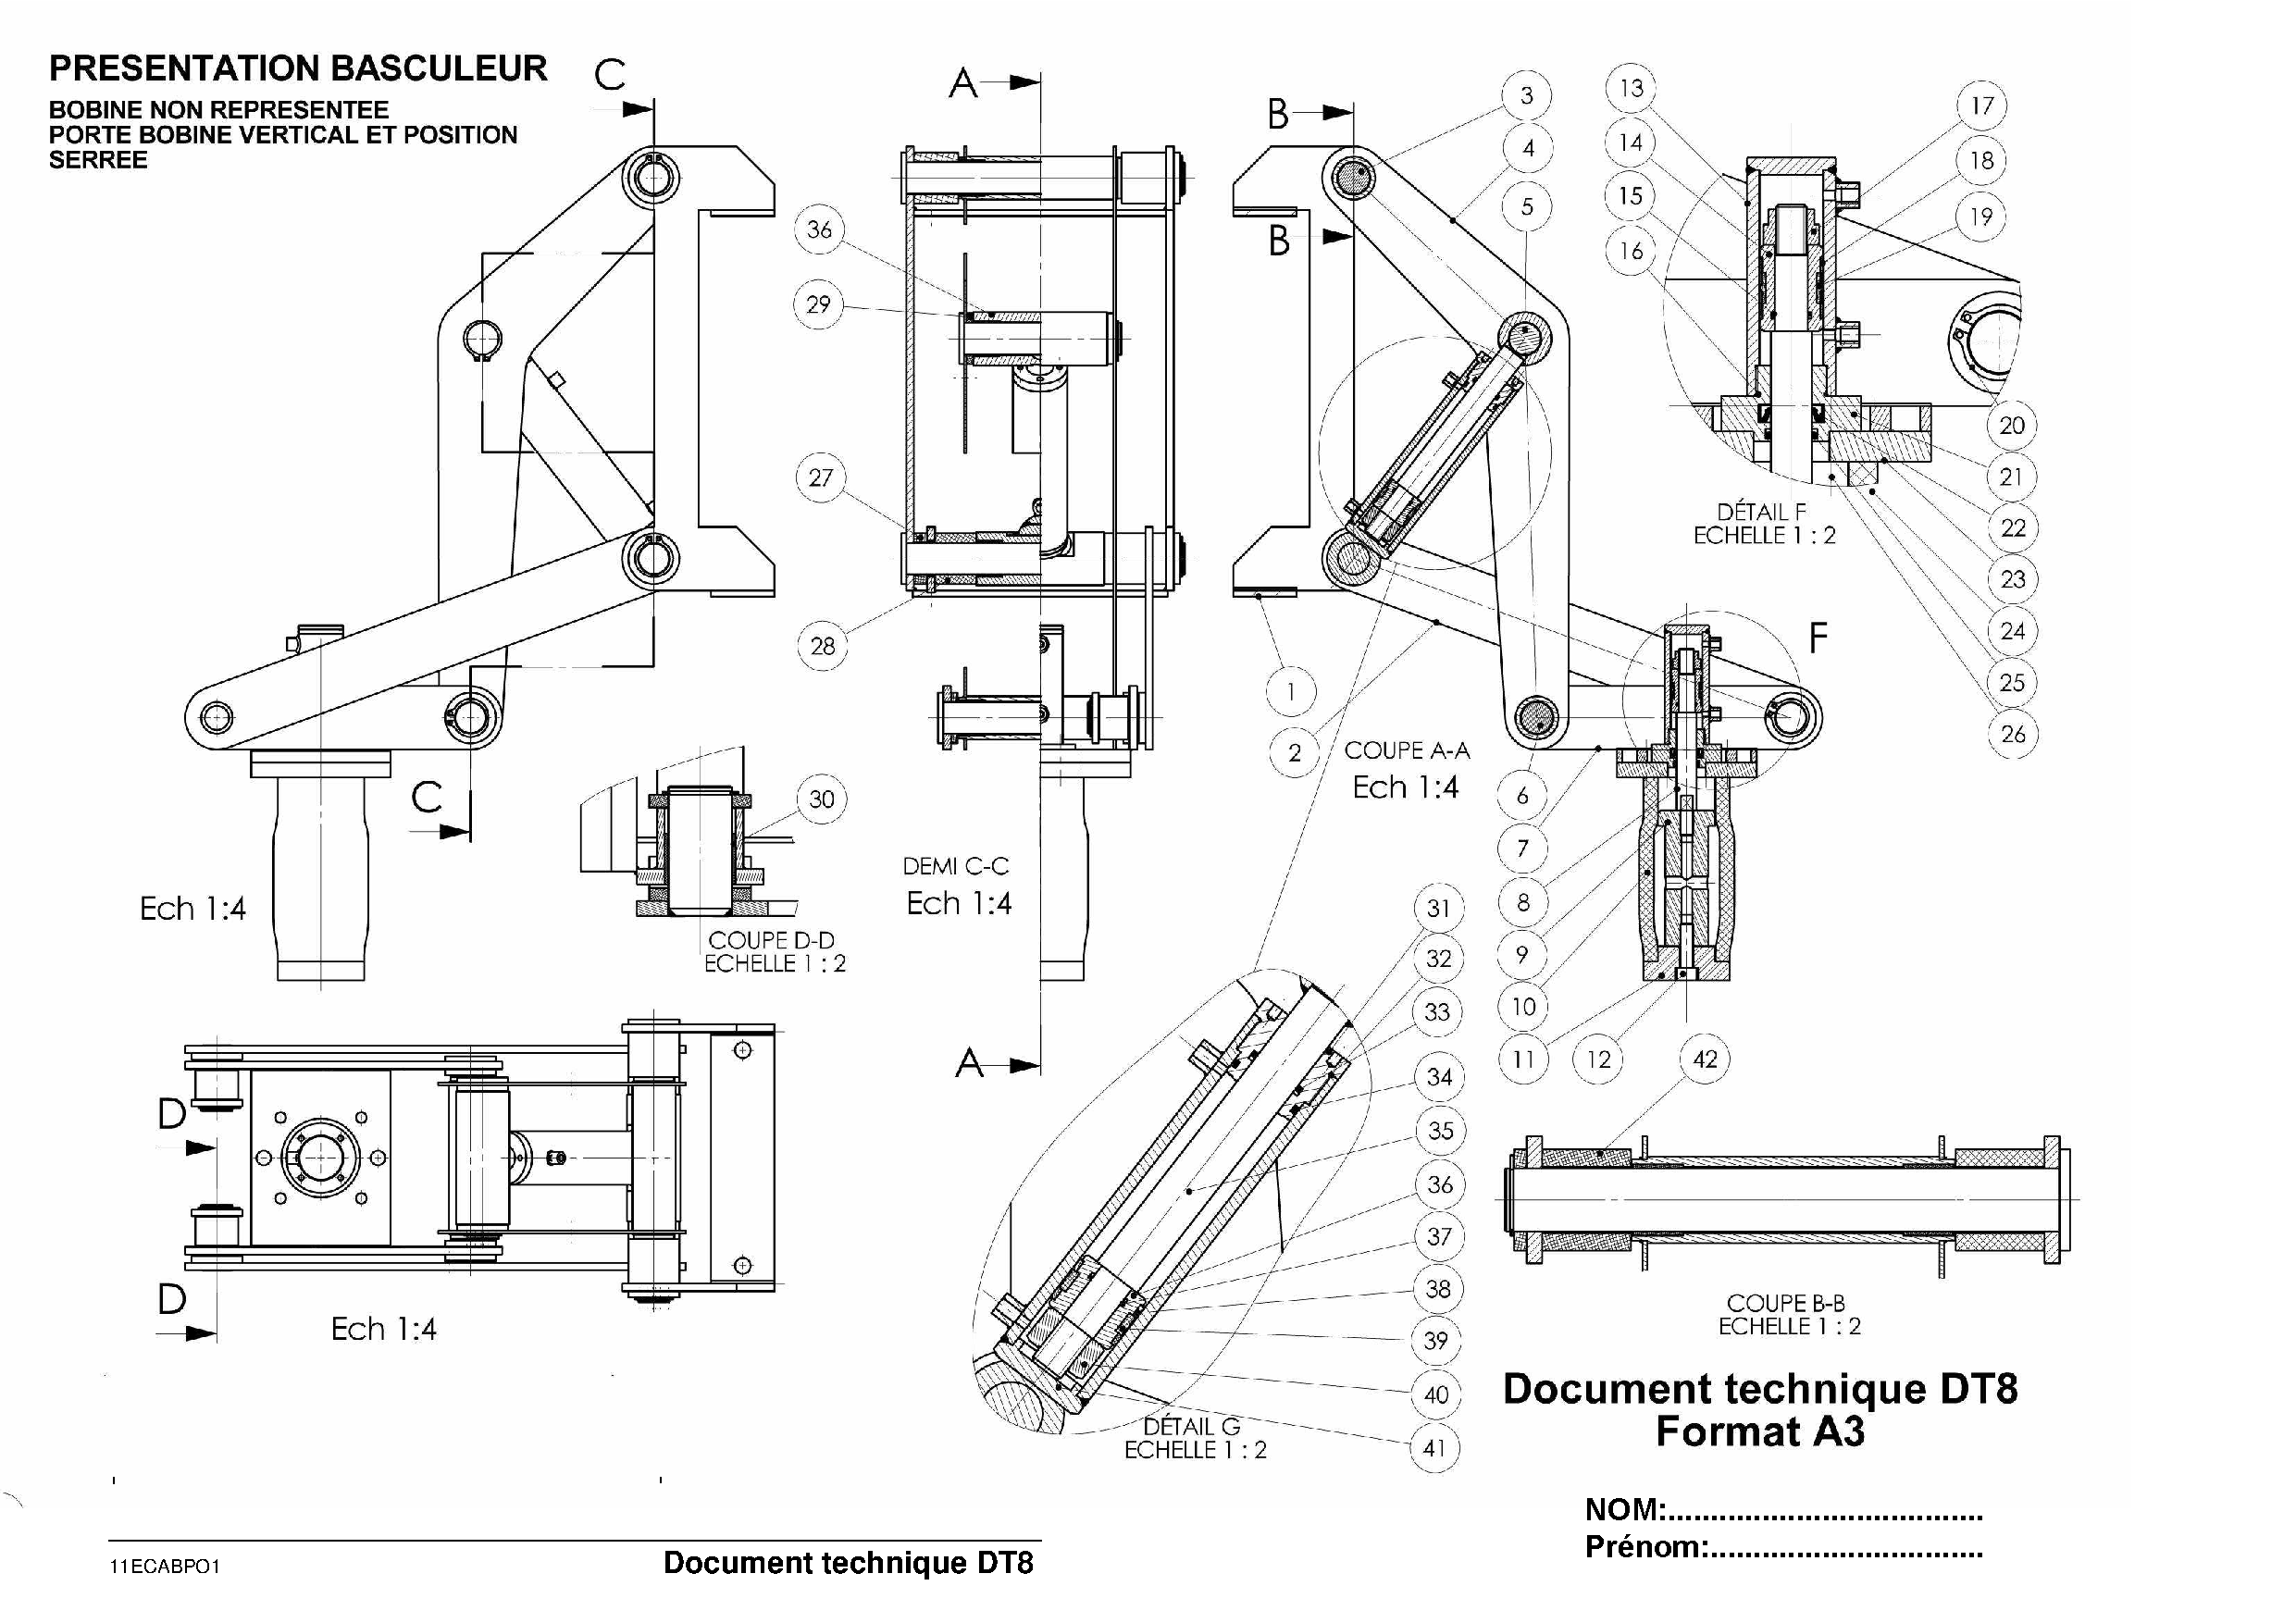
\includepdf[offset=5mm 10mm 0mm 0mm,angle=90,pages=1]{img/dessin.pdf}}{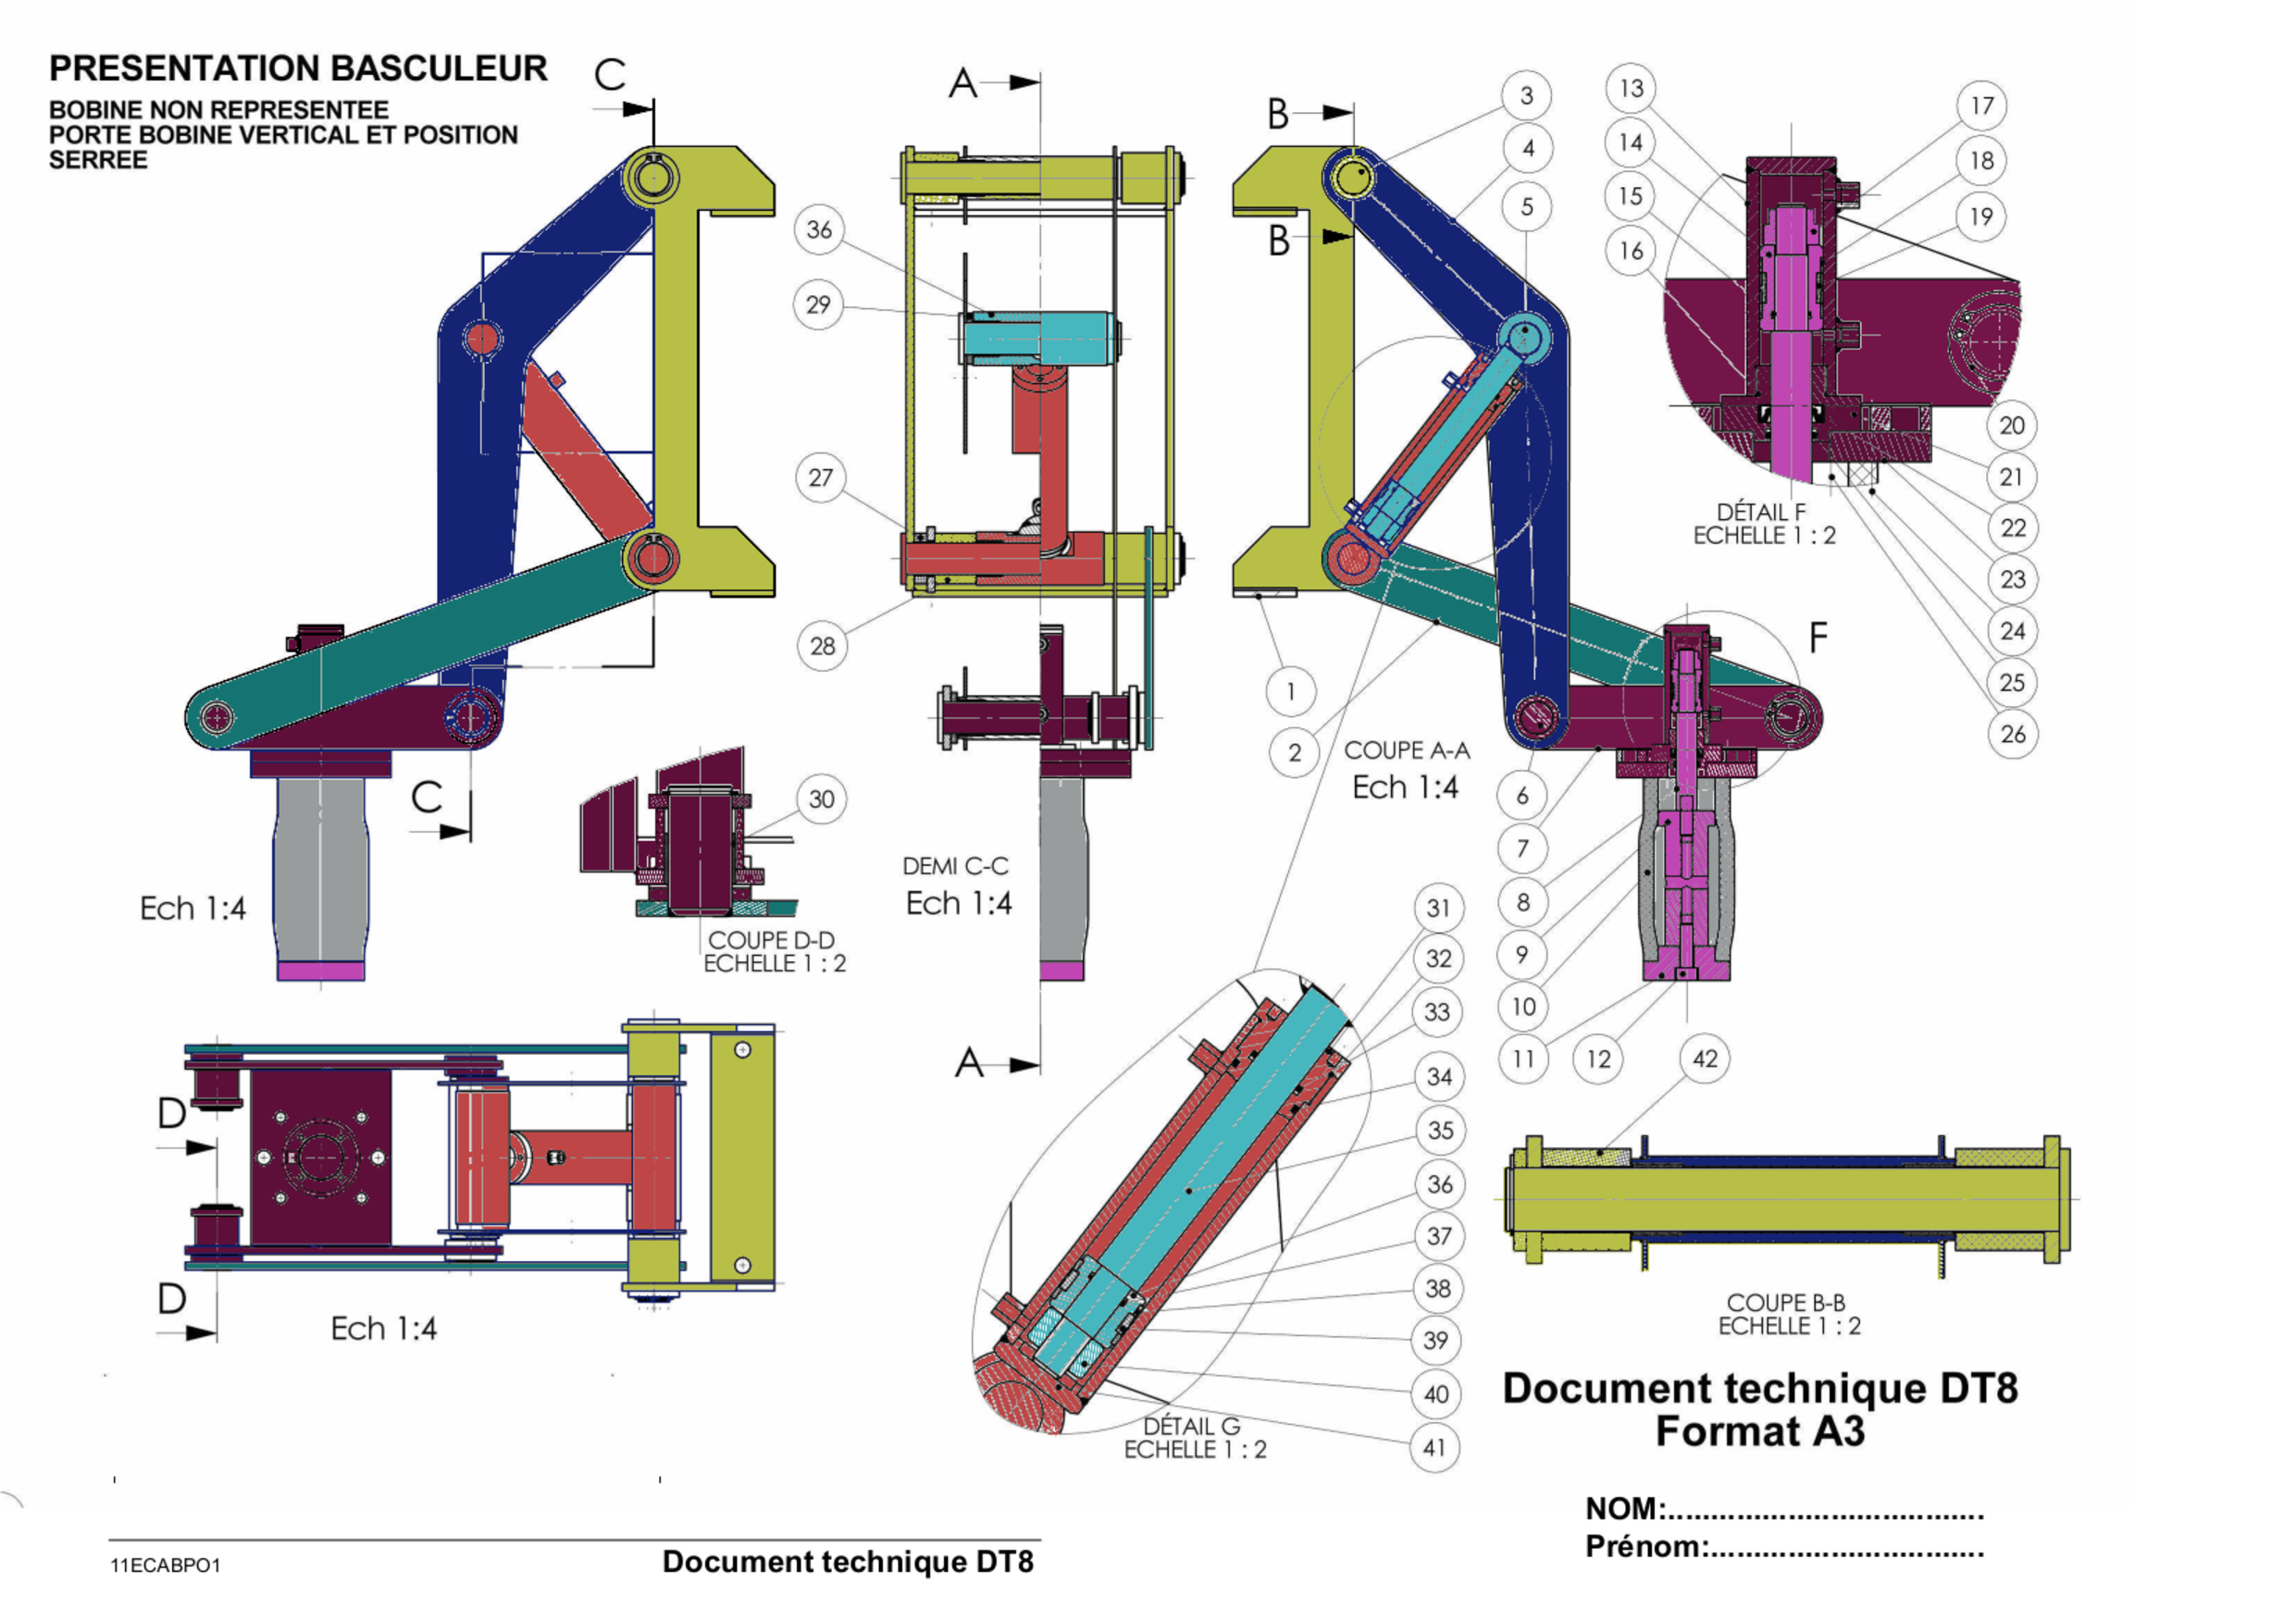
\includepdf[offset=5mm 10mm 0mm 0mm,angle=90,pages=1]{img/dessin_cor.pdf}}

\end{document}

